\chapter{Metodología}
\label{chap:metodologia}

El capítulo describe los procedimientos ejecutados para construir las representaciones tridimensionales, definir y entrenar los clasificadores clásicos, configurar Net5 y comparar los modelos conservados. Se presentan las entradas, transformaciones y criterios de validación en el orden del flujo experimental. La comprobación geométrica se distingue de la evaluación de clasificación y de las mediciones de recursos; los resultados cuantitativos se desarrollan en el capítulo siguiente.

\section{Construcción y comparación inicial de representaciones tridimensionales}\label{sec:construccion-representaciones}

En esta sección se describe la primera etapa metodológica asociada al primer objetivo específico: la construcción de la representación octree que servirá como base del enfoque clásico de clasificación tridimensional. Para verificar su implementación y caracterizar su comportamiento computacional, se construyó también una rejilla densa de referencia a partir de las mismas mallas y bajo condiciones comunes de muestreo. Ambas representaciones se generaron con resoluciones equivalentes de $32^3$ y $64^3$. Finalmente, se definió el protocolo empleado para comprobar la correspondencia entre ambas discretizaciones y comparar su estructura, almacenamiento y tiempo de construcción.

Una representación jerárquica organiza el espacio mediante subdivisiones sucesivas, de modo que su estructura se concentra en las regiones que requieren ser representadas~\parencite{samet}. En este proyecto se implementó un octree con poda por ocupación: los octantes vacíos no se materializaron como nodos, mientras que los octantes ocupados se subdividieron recursivamente hasta una profundidad máxima común. Por tanto, la estructura obtenida corresponde a una jerarquía dispersa con relaciones padre--hijo explícitas y no a una colección de rejillas independientes a diferentes resoluciones. La profundidad máxima, el número de muestras superficiales y los atributos almacenados en cada nodo se establecieron como parámetros de implementación del proyecto.

La Figura~\ref{fig:flujo} resume el flujo de procesamiento implementado. Cada malla fue leída y normalizada, y posteriormente se muestreó su superficie para obtener una nube de puntos con sus correspondientes normales. A partir de esta entrada común se desarrollaron dos rutas: la primera realizó una cuantización directa para generar la rejilla densa de referencia, mientras que la segunda construyó el octree mediante subdivisión recursiva y poda por ocupación. A continuación, se presentan la configuración experimental común, la preparación geométrica, la construcción de ambas representaciones y, finalmente, el protocolo establecido para su comparación.

\begin{figure}[H]\centering
\FiguraMetodologia{0.96\textwidth}{flujo}
\caption{Flujo de procesamiento desde las mallas OFF hasta las representaciones densa y jerárquica con resoluciones equivalentes de $32^3$ y $64^3$. Para cada objeto, ambas rutas emplearon la misma nube de $20\,000$ puntos y sus correspondientes normales. Elaboración propia.}
\label{fig:flujo}
\end{figure}

\subsection{Definición del experimento y configuración común}
\label{subsec:experimento-inicial}

Se utilizó ModelNet40\footnote{El conjunto de datos puede consultarse y descargarse desde el sitio oficial de Princeton ModelNet: \url{https://modelnet.cs.princeton.edu/}.}, un conjunto de modelos CAD tridimensionales introducido por Wu y colaboradores, cuya distribución oficial organiza los archivos por categoría y establece particiones independientes de entrenamiento y prueba~\parencite{wu2015}. El conjunto contiene $12\,311$ objetos pertenecientes a 40 clases: $9\,843$ destinados al entrenamiento y $2\,468$ a la prueba. Esta organización se conservó durante el procesamiento, aunque en esta etapa se construyeron únicamente las representaciones geométricas, sin ejecutar procedimientos de clasificación.

La ejecución documentada en esta etapa se acotó a una muestra controlada de 10 modelos: un objeto de entrenamiento y uno de prueba de cada una de las categorías \textit{airplane}, \textit{car}, \textit{chair}, \textit{sofa} y \textit{table}. Se conservaron las particiones oficiales, sin reasignar objetos entre entrenamiento y prueba. Cada modelo se procesó en $32^3$ y $64^3$, por lo que la unidad de registro fue el par modelo--resolución y se obtuvieron 20 registros. Esta muestra se utilizó para verificar el procedimiento computacional y su trazabilidad; no constituye una evaluación exhaustiva ni una muestra estadísticamente representativa de las 40 clases.

Los identificadores seleccionados fueron \protect\path{airplane_0001}, \protect\path{car_0001}, \protect\path{chair_0001}, \protect\path{sofa_0001} y \protect\path{table_0001} en entrenamiento, y \protect\path{airplane_0627}, \protect\path{car_0198}, \protect\path{chair_0890}, \protect\path{sofa_0681} y \protect\path{table_0393} en prueba, respectivamente. La evidencia de esta ejecución se conservó en la carpeta \protect\path{resultados/objetivo1/muestra_controlada/} del repositorio. Los conteos globales de ModelNet40 describen el conjunto de origen y no el alcance de la ejecución realizada.

Se seleccionaron las resoluciones equivalentes $R=32$ y $R=64$, donde
$R$ representa el número de divisiones por eje en el nivel de máxima
profundidad. Las relaciones entre el nivel del árbol, la resolución
equivalente, la profundidad máxima y la longitud del lado de las celdas
se expresan mediante las Ecuaciones~\eqref{eq:resolucion-nivel},
\eqref{eq:profundidad-maxima} y \eqref{eq:lado-celda}, respectivamente.
Estas definiciones permitieron utilizar una nomenclatura común para la
rejilla densa y el octree adaptativo.

\begin{subequations}\label{eq:niveles}
\begin{align}
R_L &= 2^L,
\label{eq:resolucion-nivel}\\
L_{\max} &= \log_2 R,
\label{eq:profundidad-maxima}\\
h_L &= \frac{2}{2^L}.
\label{eq:lado-celda}
\end{align}
\end{subequations}

En estas expresiones, $L$ denota la profundidad de un nodo,
$R_L$ corresponde a la resolución equivalente por eje en dicho nivel,
$L_{\max}$ es la profundidad máxima asociada con la resolución objetivo
$R$, y $h_L$ representa la longitud del lado de una celda en el dominio
normalizado. Puesto que la raíz cubre el dominio $[-1,1]^3$, cuyo lado
mide dos unidades normalizadas, se obtiene $h_0=2$. En consecuencia,
$R=32$ corresponde a $L_{\max}=5$ y $h_5=1/16$, mientras que $R=64$
corresponde a $L_{\max}=6$ y $h_6=1/32$.

Para cada objeto se generó una nube de $20\,000$ puntos muestreados sobre la superficie de la malla. Esta cantidad se estableció como una condición experimental común y no como el resultado de un análisis de sensibilidad. A partir de una misma nube se construyeron las representaciones densa y jerárquica en las dos resoluciones consideradas. De esta manera, las diferencias observadas entre las representaciones no pueden atribuirse al uso de muestras superficiales distintas. En esta etapa no se aplicaron rotaciones aleatorias ni otras transformaciones de aumento de datos.

Se distinguieron dos procedimientos de ejecución. En la validación ilustrativa individual con \protect\path{chair_0001.off} se utilizó directamente la semilla 42. Para el procesamiento por lotes, aplicado a la muestra controlada de 10 modelos, se adoptó igualmente 42 como semilla base, pero se derivó una semilla específica para cada objeto mediante el hash SHA-256 de su ruta relativa. En particular, se interpretaron los cuatro primeros bytes del hash como un entero sin signo de 32 bits y se sumaron a la semilla base mediante aritmética módulo $2^{32}$. Este procedimiento hizo que el muestreo de cada objeto fuera reproducible e independiente del orden de enumeración, del número de procesos y del sistema operativo.

La Tabla~\ref{tab:configuracion} resume los parámetros comunes y el entorno computacional declarado para esta etapa.
\begin{table}[H]
\centering
\small
\caption{Configuración común para la construcción y validación de las representaciones tridimensionales. Elaboración propia.}
\label{tab:configuracion}
\begin{tabularx}{\textwidth}{@{}lX@{}}
\toprule
Parámetro & Valor o condición \\
\midrule
Conjunto de datos & ModelNet40; 40 clases; $9\,843$ objetos de entrenamiento y $2\,468$ de prueba \\
Dominio normalizado & $[-1,1]^3$, cubo de lado dos \\
Resoluciones y profundidades & $32^3$: $L_{\max}=5$; $64^3$: $L_{\max}=6$ \\
Muestras por objeto & $20\,000$ puntos con las normales de sus caras de origen \\
Aumento geométrico & No se aplicaron rotaciones aleatorias ni otras transformaciones \\
Caso ilustrativo individual & Semilla 42 para \protect\path{chair_0001.off} \\
Muestra controlada & 10 modelos: cinco de entrenamiento y cinco de prueba; dos resoluciones por modelo \\
Muestreo por lotes & Semilla base 42 y semilla específica por objeto derivada mediante SHA-256 de su ruta relativa \\
Representaciones por objeto & Una rejilla densa y un octree adaptativo en cada resolución, construidos a partir de la misma nube \\
Procesador y memoria & AMD Ryzen 7 5700X; 32 GB de RAM \\
Tarjeta gráfica & NVIDIA GeForce RTX 5070 de 12 GB; no utilizada en esta etapa \\
Entorno declarado & Windows 11; Python 3.14.4; NumPy 2.4.6 \\
Procesamiento & Operaciones geométricas ejecutadas en CPU; número de procesos configurable \\
\bottomrule
\end{tabularx}
\end{table}

La nube de puntos se generó una sola vez por objeto y se reutilizó para construir las representaciones en $32^3$ y $64^3$. El número de procesos paralelos modificó únicamente la distribución de las tareas y no las semillas asignadas ni las representaciones resultantes. Los registros del caso ilustrativo individual y de la muestra controlada se interpretaron por separado, puesto que sus mecanismos de asignación de semillas no producen necesariamente las mismas muestras superficiales.

Se utilizó \protect\path{chair_0001.off}, perteneciente a la categoría \textit{chair}, como caso ilustrativo para verificar la lectura, la transformación espacial, el muestreo superficial, la ocupación y la conservación de la jerarquía. El archivo contiene $2\,382$ vértices y $2\,234$ caras procesadas. Las ilustraciones correspondientes a este caso se generaron con $20\,000$ puntos y semilla 42. Por tanto, sus conteos y características corresponden exclusivamente a este objeto y no se presentan como resultados generales de ModelNet40.

\subsection{Preparación geométrica de la malla}
\label{subsec:preparacion-malla}

Los archivos OFF se leyeron mediante la función \protect\path{leer_off}. De cada archivo se obtuvieron las coordenadas de los vértices y los índices de las caras en arreglos de formas $(N_v,3)$ y $(N_f,3)$, con tipos \texttt{float32} e \texttt{int64}, respectivamente. En esta notación, $N_v$ representa el número de vértices y $N_f$ el número de caras conservadas después de la lectura. La conectividad de la malla se utilizó para identificar los triángulos durante el muestreo; la nube de puntos generada posteriormente contiene muestras de la superficie y no conserva dicha conectividad.

Las coordenadas no finitas de los vértices se sustituyeron por cero y se descartaron las caras cuyos índices se encontraban fuera del intervalo válido. Para cada registro de cara que pudo ser interpretado por el lector se conservaron únicamente los tres primeros índices. Por consiguiente, este procedimiento no realizó una triangulación general de caras poligonales y asumió registros compatibles con la lectura empleada. Tampoco se aplicaron procedimientos de reparación topológica ni verificaciones de cierre, orientación global o ausencia de autointersecciones. Los fallos de lectura se gestionaron mediante el registro de excepciones por objeto; las sustituciones de coordenadas y los descartes de caras realizados internamente por el lector no se contabilizaron de forma independiente.

Los vértices se centraron y se escalaron mediante un único factor para llevar cada objeto al dominio espacial común. La media de los vértices, el factor de escala y las coordenadas normalizadas se definieron mediante las Ecuaciones~\eqref{eq:centro-vertices}, \eqref{eq:factor-escala} y \eqref{eq:vertices-normalizados}, respectivamente.

\begin{subequations}\label{eq:normalizacion}
\begin{align}
\mathbf c
&=
\frac{1}{N_v}
\sum_{a=1}^{N_v}\mathbf v_a,
\label{eq:centro-vertices}\\
s
&=
\max_{\substack{1\leq a\leq N_v\\k\in\{x,y,z\}}}
\left|v_{a,k}-c_k\right|,
\label{eq:factor-escala}\\
\widetilde{\mathbf v}_a
&=
\begin{cases}
\dfrac{\mathbf v_a-\mathbf c}{s}, & s>0,\\[2mm]
\mathbf v_a-\mathbf c, & s=0.
\end{cases}
\label{eq:vertices-normalizados}
\end{align}
\end{subequations}

En estas expresiones, $\mathbf v_a$ representa el vértice original de índice $a$, $N_v$ es el número de vértices, $\mathbf c$ corresponde a la media aritmética de sus coordenadas, $v_{a,k}$ y $c_k$ denotan las componentes del vértice y de la media sobre el eje $k\in\{x,y,z\}$, y $s$ es la máxima desviación absoluta respecto a $\mathbf c$. Finalmente, $\widetilde{\mathbf v}_a$ representa el vértice normalizado.

Cuando $s>0$, la transformación garantiza que todas las coordenadas normalizadas pertenezcan al intervalo $[-1,1]$. Si $s=0$, todos los vértices coinciden y únicamente se aplica el centrado para evitar una división por cero. La media de los vértices se empleó como centro de la transformación; por tanto, no corresponde al centroide ponderado por el área de la superficie. Debido a que se utilizó un único factor escalar
para los tres ejes, se conservaron las proporciones originales de la malla. No se aplicó ninguna transformación adicional de rotación o alineación.

La Figura~\ref{fig:mallas} muestra el objeto antes y después de esta transformación. Durante la normalización se modificaron las coordenadas de los vértices, pero se mantuvieron los índices que definen las caras.
\begin{figure}[htbp]
\centering
\begin{subfigure}[t]{.48\textwidth}
\centering
\FiguraMetodologia{\linewidth}{mallas_a}
\caption{Malla original.}\label{fig:malla-original}
\end{subfigure}
\hfill
\begin{subfigure}[t]{.48\textwidth}
\centering
\FiguraMetodologia{\linewidth}{mallas_b}
\caption{Malla normalizada.}\label{fig:malla-normalizada}
\end{subfigure}
\caption{\textbf{(a)} Malla original y \textbf{(b)} malla normalizada de \protect\path{chair_0001}. La transformación se realizó antes de construir las representaciones en $32^3$ y $64^3$; en esta etapa todavía no existe discretización volumétrica. Elaboración propia.}
\label{fig:mallas}
\end{figure}

Para generar la nube de puntos se seleccionaron las caras con una
probabilidad proporcional a su área. El muestreo uniforme dentro de
cada triángulo se fundamentó en la transformación de coordenadas
baricéntricas descrita por Pharr, Jakob y
Humphreys~\parencite{pbrt}. El área de cada cara triangular y su
probabilidad de selección se definieron mediante las
Ecuaciones~\eqref{eq:area-cara} y \eqref{eq:probabilidad-cara},
respectivamente.

\begin{subequations}\label{eq:areas}
\begin{align}
A_t
&=
\frac{1}{2}
\left\|
(\mathbf b_t-\mathbf a_t)
\times
(\mathbf c_t-\mathbf a_t)
\right\|_2,
\label{eq:area-cara}\\
\pi_t
&=
\frac{A_t}
{\displaystyle\sum_{j=1}^{N_f}A_j},
\qquad
\sum_{j=1}^{N_f}A_j>0.
\label{eq:probabilidad-cara}
\end{align}
\end{subequations}

En estas expresiones, $\mathbf a_t$, $\mathbf b_t$ y $\mathbf c_t$
son los tres vértices normalizados de la cara triangular $t$;
$A_t$ representa su área en unidades normalizadas al cuadrado;
$N_f$ es el número de caras conservadas después de la lectura; y
$\pi_t$ corresponde a la probabilidad de seleccionar la cara $t$.
El índice $j$ recorre las $N_f$ caras procesadas. A partir de la
distribución definida por $\{\pi_t\}_{t=1}^{N_f}$, se seleccionaron
$20\,000$ índices de cara con reemplazo, por lo que una misma cara
podía ser seleccionada más de una vez. La ponderación por área evitó
asignar la misma probabilidad a triángulos de tamaños diferentes y
permitió que la frecuencia esperada de muestras sobre cada cara fuera
proporcional a su extensión superficial.

Después de seleccionar una cara, se generaron dos variables aleatorias uniformes independientes y se obtuvo el punto sobre su superficie mediante la Ecuación~\eqref{eq:muestreo}~\parencite{pbrt}.
\begin{equation}
\mathbf p_i=
(1-\sqrt{u_i})\mathbf a_t
+
\sqrt{u_i}(1-v_i)\mathbf b_t
+
\sqrt{u_i}v_i\mathbf c_t,
\qquad
u_i,v_i\sim\mathcal U(0,1).
\label{eq:muestreo}
\end{equation}
Aquí, $i\in\{1,\ldots,N_p\}$ identifica la muestra, $N_p=20\,000$, $t$ es la cara seleccionada y $\mathbf p_i$ es el punto normalizado resultante. Los tres coeficientes de la combinación son baricéntricos, no negativos y suman uno. Bajo aritmética ideal, esta transformación produce una distribución uniforme respecto al área de cada triángulo. Sin embargo, por tratarse de un muestreo finito, no se garantiza que todas las celdas intersectadas por la superficie reciban al menos una muestra.

A cada punto se le asignó la normal de la cara triangular de la cual
fue generado. Primero se calculó el vector normal no normalizado de
la cara mediante la Ecuación~\eqref{eq:vector-normal-cara}.
Posteriormente, este vector se normalizó de acuerdo con la
Ecuación~\eqref{eq:normal-muestra}. Para evitar divisiones por cero o
por valores numéricamente insignificantes, se fijó el umbral
$\varepsilon=10^{-12}$.

\begin{subequations}\label{eq:normalcara}
\begin{align}
\mathbf w_t
&=
(\mathbf b_t-\mathbf a_t)
\times
(\mathbf c_t-\mathbf a_t),
\label{eq:vector-normal-cara}\\
\mathbf n_i
&=
\frac{\mathbf w_t}
{\max\left(\|\mathbf w_t\|_2,\varepsilon\right)}.
\label{eq:normal-muestra}
\end{align}
\end{subequations}

En estas expresiones, $\mathbf w_t$ es el vector normal no normalizado
obtenido mediante el producto cruz de dos lados de la cara $t$, y
$\mathbf n_i$ es la normal asignada a la muestra $\mathbf p_i$
generada sobre dicha cara. Cuando
$\|\mathbf w_t\|_2>\varepsilon$, el vector resultante tiene norma
unitaria. El umbral $\varepsilon$ evita la división por cero; en
particular, una cara degenerada con $\mathbf w_t=\mathbf 0$ produce
una normal nula. La orientación de $\mathbf n_i$ depende del orden de
los vértices de la cara. No se interpolaron normales de vértice ni se
corrigió globalmente la orientación de las caras.

Cuando una malla no contenía caras válidas o cuando la suma de sus áreas no era positiva, la implementación utilizó un procedimiento alternativo: se seleccionaron vértices de la malla y se asignaron normales nulas a las muestras obtenidas. Este comportamiento corresponde a una ruta de contingencia de la implementación y se distingue del muestreo superficial ponderado por área.

La Figura~\ref{fig:nube} presenta la nube obtenida para el caso ilustrativo. Como resultado se conservaron dos arreglos \texttt{float32} de forma $(20\,000,3)$: uno con las posiciones y otro con las normales. Los mismos arreglos se utilizaron para construir la rejilla densa y el octree adaptativo en ambas resoluciones.
\begin{figure}[H]
\centering
\FiguraMetodologia{0.66\textwidth}{nube}
\caption{Nube de $20\,000$ puntos obtenida de \protect\path{chair_0001}, después de la normalización y el muestreo con semilla 42. Esta nube constituye la entrada común para las representaciones en $32^3$ y $64^3$; no corresponde todavía a una rejilla ni a un octree. Elaboración propia.}
\label{fig:nube}
\end{figure}

\subsection{Voxelización densa}
\label{subsec:voxelizacion-densa}

La rejilla densa se construyó directamente a partir de los puntos normalizados mediante la función \protect\path{construir_grid_octree}, pese al nombre histórico de esta función. Esta ruta no utilizó como entrada un árbol construido previamente. Una representación regular permite asociar información a celdas volumétricas~\parencite{wu2015}; en la implementación correspondiente al primer objetivo específico se adoptó una ocupación determinada por la presencia de muestras superficiales, sin rellenar el interior del objeto.

La Ecuación~\eqref{eq:indices} define la asignación de cada coordenada a un índice válido de la rejilla.
\begin{equation}
j_{i,k}=
\min\left(
R-1,
\max\left(
0,
\left\lfloor
\frac{p_{i,k}+1}{2}R
\right\rfloor
\right)
\right).
\label{eq:indices}
\end{equation}
El índice $j_{i,k}\in\{0,\ldots,R-1\}$ corresponde al eje $k$ del punto $\mathbf p_i$, mientras que $\lfloor\cdot\rfloor$ denota la función piso. La transformación se aplicó a los tres ejes. El recorte incorporó los puntos situados en el borde superior del dominio a la última celda de la rejilla. Para los valores no negativos obtenidos después de transformar el dominio $[-1,1]^3$, la conversión al tipo entero realizada por el código es equivalente a la aplicación de la función piso.

Los puntos que recibieron el mismo índice tridimensional se agruparon en una misma celda. Las Ecuaciones~\eqref{eq:ocupacion-muestras}--\eqref{eq:ocupacion-indicador} definen, respectivamente, el conjunto de muestras de la celda, su número de muestras y el indicador de ocupación.
\begin{subequations}\label{eq:ocupacion}
\begin{align}
I_{\mathbf j}&=\{i:(j_{i,x},j_{i,y},j_{i,z})=\mathbf j\}, \label{eq:ocupacion-muestras} \\
m_{\mathbf j}&=|I_{\mathbf j}|, \label{eq:ocupacion-conteo} \\
O_{\mathbf j}&=\mathbf1[m_{\mathbf j}>0]. \label{eq:ocupacion-indicador}
\end{align}
\end{subequations}
En estas expresiones, $\mathbf j$ es el índice tridimensional de una celda, $I_{\mathbf j}$ es el conjunto de muestras asignadas a ella, $m_{\mathbf j}$ es su número de muestras y $\mathbf 1[\cdot]$ es la función indicadora. Una celda se marcó como ocupada cuando recibió al menos un punto. Por tanto, este criterio representa la discretización de la nube muestreada y no constituye una prueba geométrica exacta de intersección entre los triángulos de la malla y las celdas de la rejilla.

Las Ecuaciones~\eqref{eq:promedio-normal-celda}--\eqref{eq:normal-celda-normalizada} definen el promedio de las normales de las muestras asignadas a cada celda y su normalización posterior, respectivamente. Se utilizó el umbral $\varepsilon=10^{-12}$ definido previamente.

\begin{subequations}\label{eq:normalcelda}
\begin{align}
\overline{\mathbf n}_{\mathbf j}
&=
\frac{
\displaystyle\sum_{i\in I_{\mathbf j}}\mathbf n_i
}{
\max(m_{\mathbf j},1)
},
\label{eq:promedio-normal-celda}\\
\widehat{\mathbf n}_{\mathbf j}
&=
\begin{cases}
\dfrac{\overline{\mathbf n}_{\mathbf j}}
{\|\overline{\mathbf n}_{\mathbf j}\|_2},
&
\|\overline{\mathbf n}_{\mathbf j}\|_2>\varepsilon,\\[2mm]
\mathbf 0,
&
\text{en otro caso}.
\end{cases}
\label{eq:normal-celda-normalizada}
\end{align}
\end{subequations}

En estas expresiones, $\overline{\mathbf n}_{\mathbf j}$ representa
el promedio de las normales de las muestras asignadas a la celda
$\mathbf j$, mientras que $\widehat{\mathbf n}_{\mathbf j}$
corresponde a su versión normalizada. El término
$\max(m_{\mathbf j},1)$ evita la división por cero en las celdas
vacías, y el umbral $\varepsilon=10^{-12}$ es consistente con el
utilizado durante el cálculo de las normales de las caras. Las celdas
vacías y aquellas cuyo vector promedio presentó una norma inferior o
igual que dicho umbral recibieron una normal nula. En consecuencia,
una celda ocupada también pudo contener una normal nula cuando las
orientaciones de sus muestras se cancelaron durante el promedio.
Finalmente, la ocupación y las tres componentes de la normal
normalizada,
$\left[O_{\mathbf j},
\widehat n_{\mathbf j,x},
\widehat n_{\mathbf j,y},
\widehat n_{\mathbf j,z}\right]$,
se almacenaron en un arreglo de tipo \texttt{float32} y forma
$(4,R,R,R)$.

El Algoritmo~\ref{alg:densa} resume la construcción independiente de la rejilla densa y explicita sus entradas, parámetros y salida.
\begin{algorithm}[H]
\caption{Construcción directa de la rejilla densa.}
\label{alg:densa}
\begin{algorithmic}[1]
\Require Puntos $P=(\mathbf p_i)$ y normales $N=(\mathbf n_i)$; $N_p=20\,000$; $R\in\{32,64\}$; $\varepsilon=10^{-12}$.
\Ensure Tensor $G\in\mathbb R^{4\times R\times R\times R}$ en \texttt{float32}.
\State Reservar los conteos y las sumas de normales, inicializados en cero.
\For{cada muestra $i=1,\ldots,N_p$}
    \State Calcular $\mathbf j_i$ mediante la Ecuación~\eqref{eq:indices}.
    \State Incrementar el conteo de $\mathbf j_i$ y sumar $\mathbf n_i$.
\EndFor
\State Obtener la ocupación mediante las Ecuaciones~\eqref{eq:ocupacion-muestras}--\eqref{eq:ocupacion-indicador}.
\State Calcular y normalizar los promedios mediante las Ecuaciones~\eqref{eq:promedio-normal-celda}--\eqref{eq:normal-celda-normalizada}.
\State Concatenar la ocupación y las tres componentes de la normal en $G$.
\State \Return $G$.
\end{algorithmic}
\end{algorithm}

La implementación de \texttt{octree.py} acumuló los conteos y las componentes de las normales mediante índices lineales y operaciones vectorizadas de NumPy. Las etapas conceptuales del algoritmo corresponden a cuantización, acumulación, normalización y concatenación; ninguna de ellas requiere materializar un octree. Para estimar el tamaño de almacenamiento, el tensor se guardó temporalmente en formato NPZ comprimido después de su construcción. El tiempo requerido para esta escritura no se incluyó en el tiempo de construcción de la rejilla densa.

La Figura~\ref{fig:rejillas} presenta las celdas ocupadas del caso ilustrativo en las dos resoluciones. Las celdas vacías se ocultaron para permitir la observación de la geometría, aunque el arreglo denso reservó espacio para todas las celdas del dominio.
\begin{figure}[htbp]
\centering
\begin{subfigure}[t]{.48\textwidth}
\centering
\FiguraMetodologia{\linewidth}{rejillas_a}
\caption{Rejilla de resolución $32^3$.}\label{fig:rejilla32}
\end{subfigure}
\hfill
\begin{subfigure}[t]{.48\textwidth}
\centering
\FiguraMetodologia{\linewidth}{rejillas_b}
\caption{Rejilla de resolución $64^3$.}\label{fig:rejilla64}
\end{subfigure}
\caption{Voxelización directa de la nube de puntos de \protect\path{chair_0001}: \textbf{(a)} rejilla de resolución $32^3$, con 762 celdas ocupadas; y \textbf{(b)} rejilla de resolución $64^3$, con $2\,573$ celdas ocupadas. La visualización presenta únicamente las celdas ocupadas, aunque los arreglos densos reservan espacio para todas las celdas. Elaboración propia.}
\label{fig:rejillas}
\end{figure}

El tamaño teórico de los datos del tensor se calculó considerando
$C=4$ canales y $b=4$ bytes por cada elemento de tipo
\texttt{float32}. Como la rejilla contiene $R^3$ celdas, el número
total de bytes se determinó mediante las Ecuaciones~\eqref{eq:bytesdenso-general}--\eqref{eq:bytesdenso-float32}, de forma independiente del consumo
transitorio requerido durante su construcción.

\begin{subequations}\label{eq:bytesdenso}
\begin{align}
B_D&=C R^3 b, \label{eq:bytesdenso-general} \\
B_D&=16R^3\ \text{bytes}. \label{eq:bytesdenso-float32}
\end{align}
\end{subequations}

En estas expresiones, $B_D$ representa el tamaño de los datos del arreglo,
$C$ es el número de canales, $R^3$ es el número total de celdas de la
rejilla y $b$ es el número de bytes ocupado por cada elemento. Para
$R=32$ se obtuvo
$B_D=524\,288$ bytes, equivalentes a 512~KiB, mientras que para
$R=64$ se obtuvieron $4\,194\,304$ bytes, equivalentes a 4~MiB.
Estas cantidades excluyen los metadatos de Python, los arreglos
temporales empleados durante la construcción y los efectos de la
compresión. Por tanto, se utilizaron como referencia teórica del
almacenamiento requerido por los datos de la representación regular.

\subsection{Construcción de la representación jerárquica mediante octree adaptativo}
\label{subsec:octree-adaptativo}

Se construyó una instancia de \texttt{NodoOctree} como nodo raíz, con centro $\mathbf{0}$, lado dos y profundidad $L=0$. La subdivisión del espacio en ocho octantes siguió la organización jerárquica propia de los octrees~\parencite{samet}. Únicamente se crearon los hijos que recibieron puntos; las posiciones correspondientes a octantes vacíos se conservaron como referencias \texttt{None}. La adaptatividad implementada consistió en esta poda por ocupación. No se utilizaron umbrales de curvatura, error geométrico o cantidad de puntos para detener anticipadamente una rama ocupada. En consecuencia, todas las hojas ocupadas alcanzaron la profundidad $L_{\max}$.

La asignación de cada punto a uno de los ocho octantes del nodo actual se realizó en dos etapas. Primero, la Ecuación~\eqref{eq:bit-octante} determinó el semiespacio ocupado por el punto respecto al plano medio de cada eje. Después, la Ecuación~\eqref{eq:indice-octante} combinó los tres indicadores binarios para obtener el índice del octante.

\begin{subequations}\label{eq:octante}
\begin{align}
b_k
&=
\mathbf 1
\left[
p_{i,k}\geq c_{\nu,k}
\right],
\qquad
k\in\{x,y,z\},
\label{eq:bit-octante}\\
q(\mathbf p_i,\mathbf c_\nu)
&=
b_x+2b_y+4b_z.
\label{eq:indice-octante}
\end{align}
\end{subequations}

En estas expresiones, $\nu$ identifica el nodo actual, $\mathbf c_\nu$ es su centro, $\mathbf p_i$ es el punto que se clasifica y $b_k\in\{0,1\}$ indica el semiespacio determinado por el plano medio perpendicular al eje $k$. Los puntos situados exactamente sobre uno de estos planos se asignaron al semiespacio positivo debido al uso de la condición $\geq$ en la Ecuación~\eqref{eq:bit-octante}. El valor $q\in\{0,\ldots,7\}$ identifica el octante resultante: $b_x$ ocupa el bit cero, $b_y$ el bit uno y $b_z$ el bit dos.

Para cada octante no vacío se calcularon el centro, la longitud del
lado y la profundidad del nodo hijo. Estas propiedades se definieron
mediante las Ecuaciones~\eqref{eq:centro-hijo},
\eqref{eq:lado-hijo} y \eqref{eq:profundidad-hijo},
respectivamente.

\begin{subequations}\label{eq:hijo}
\begin{align}
\mathbf c_{\nu,q}
&=
\mathbf c_\nu
+
\frac{h_\nu}{4}
\left(
2b_x-1,\,
2b_y-1,\,
2b_z-1
\right),
\label{eq:centro-hijo}\\
h_{\nu,q}
&=
\frac{h_\nu}{2},
\label{eq:lado-hijo}\\
L_{\nu,q}
&=
L_\nu+1.
\label{eq:profundidad-hijo}
\end{align}
\end{subequations}

En estas expresiones, $\mathbf c_\nu$, $h_\nu$ y $L_\nu$
representan, respectivamente, el centro, la longitud del lado y la
profundidad del nodo padre $\nu$. El subíndice $(\nu,q)$ identifica
al hijo correspondiente al octante $q$, mientras que
$b_x$, $b_y$ y $b_z$ son los indicadores binarios definidos en la
Ecuación~\eqref{eq:bit-octante}. El centro del hijo se desplazó una
distancia $h_\nu/4$ respecto al centro del padre en cada eje, con el
signo determinado por el octante. Al mismo tiempo, la longitud de su
lado se redujo a la mitad y su profundidad se incrementó en una
unidad. Estas operaciones se aplicaron en cada llamada recursiva,
conservando las relaciones espaciales entre los nodos padres y sus
hijos.

El Algoritmo~\ref{alg:octree} resume la construcción. La entrada fue la nube normalizada, no una rejilla previamente construida. La recursión solo se ejecutó sobre octantes no vacíos y la condición de parada para las ramas ocupadas fue alcanzar la profundidad máxima.
\begin{algorithm}[H]
\caption{Construcción recursiva del octree adaptativo con poda de octantes vacíos.}
\label{alg:octree}
\begin{algorithmic}[1]
\Require Puntos $P=(\mathbf p_i)$ y normales $N=(\mathbf n_i)$, con $|P|=20\,000$; $L_{\max}\in\{5,6\}$; centro inicial $\mathbf{0}$; lado inicial $2$; nivel inicial $0$; $\varepsilon=10^{-12}$.
\Ensure Nodo raíz de un octree con relaciones padre--hijo explícitas.
\Function{Construir}{$P,N,\mathbf c,h,L$}
    \State Crear nodo $\nu$ con centro $\mathbf c$, lado $h$, nivel $L$ y ocho hijos ausentes.
    \State Marcar $\nu$ como ocupado y registrar $|P|$.
    \If{$L=L_{\max}$}
        \State Marcar $\nu$ como hoja.
        \State $\overline{\mathbf n}_\nu \gets |P|^{-1}\sum_i \mathbf n_i$.
        \State $\rho_\nu\gets\|\overline{\mathbf n}_\nu\|_2$.
        \State Almacenar $\rho_\nu$ como coherencia normal.
        \If{$\rho_\nu>\varepsilon$}
            \State $\widehat{\mathbf n}_\nu\gets\overline{\mathbf n}_\nu/\rho_\nu$.
        \Else
            \State $\widehat{\mathbf n}_\nu\gets\mathbf{0}$.
        \EndIf
        \State Almacenar $\widehat{\mathbf n}_\nu$ y \Return $\nu$.
    \EndIf
    \State Marcar $\nu$ como nodo interno y asignar los puntos a octantes mediante las Ecuaciones~\eqref{eq:bit-octante}--\eqref{eq:indice-octante}.
    \For{$q=0,\ldots,7$}
        \State Seleccionar $P_q$ y $N_q$ correspondientes al octante $q$.
        \If{$|P_q|>0$}
            \State Calcular $\mathbf c_{\nu,q}$ y $h_{\nu,q}$ mediante las Ecuaciones~\eqref{eq:centro-hijo}--\eqref{eq:lado-hijo}.
            \State $\nu.\mathrm{hijos}[q]\gets\Call{Construir}{P_q,N_q,\mathbf c_{\nu,q},h_{\nu,q},L+1}$.
        \EndIf
    \EndFor
    \State \Return $\nu$.
\EndFunction
\State \Return \Call{Construir}{$P,N,\mathbf{0},2,0$}.
\end{algorithmic}
\end{algorithm}

La función \protect\path{construir_octree} de \protect\path{octree_real.py} implementó este procedimiento. Cada nodo almacenó su centro, lado, profundidad, estado de ocupación, condición de hoja, ocho referencias a posibles hijos y el número de puntos asignados. Un octante vacío permaneció como una referencia \texttt{None}, sin reservar un objeto de tipo \texttt{NodoOctree}. Las selecciones temporales de puntos y normales realizadas durante la recursión contribuyeron al consumo máximo transitorio de memoria.

Las hojas ocupadas almacenaron dos descriptores asociados con las normales. El primero fue la dirección normal promedio normalizada, $\widehat{\mathbf n}_\nu$, calculada mediante el procedimiento definido en las Ecuaciones~\eqref{eq:promedio-normal-celda}--\eqref{eq:normal-celda-normalizada}. El segundo fue la coherencia normal, definida mediante la Ecuación~\eqref{eq:coherencia-normal}.
\begin{equation}
\rho_\nu
=
\left\|
\overline{\mathbf n}_\nu
\right\|_2,
\qquad
0\leq\rho_\nu\leq 1.
\label{eq:coherencia-normal}
\end{equation}
La coherencia normal corresponde a la magnitud del promedio de las normales antes de su normalización. Un valor cercano a uno indica que las normales asignadas a la hoja presentan direcciones semejantes, mientras que un valor cercano a cero indica dispersión o cancelación entre orientaciones. Los nodos internos no almacenaron una dirección normal ni una coherencia con significado geométrico. 

La Figura~\ref{fig:jerarquia} presenta los nodos existentes en cada nivel para el caso ilustrativo. Los paneles se obtuvieron recorriendo el árbol construido y no mediante la agregación de una rejilla densa. La raíz aparece como un único cubo y los niveles siguientes muestran progresivamente el efecto de la poda espacial. El nivel $L=5$ contiene 762 hojas ocupadas y corresponde a una resolución equivalente de $32^3$. Al extender la misma nube hasta $L=6$ se obtienen $2\,573$ hojas ocupadas, equivalentes a $64^3$. Los árboles contienen, respectivamente, $1\,121$ y $3\,694$ nodos totales.
\begin{figure}[htbp]
\centering
\begin{subfigure}[t]{.31\textwidth}
\centering
\FiguraMetodologia{\linewidth}{jerarquia_R64_a}
\caption{}\label{fig:jerarquia-nivel0}
\end{subfigure}
\hfill
\begin{subfigure}[t]{.31\textwidth}
\centering
\FiguraMetodologia{\linewidth}{jerarquia_R64_b}
\caption{}\label{fig:jerarquia-nivel1}
\end{subfigure}
\hfill
\begin{subfigure}[t]{.31\textwidth}
\centering
\FiguraMetodologia{\linewidth}{jerarquia_R64_c}
\caption{}\label{fig:jerarquia-nivel2}
\end{subfigure}
\par\medskip
\begin{subfigure}[t]{.31\textwidth}
\centering
\FiguraMetodologia{\linewidth}{jerarquia_R64_d}
\caption{}\label{fig:jerarquia-nivel3}
\end{subfigure}
\hfill
\begin{subfigure}[t]{.31\textwidth}
\centering
\FiguraMetodologia{\linewidth}{jerarquia_R64_e}
\caption{}\label{fig:jerarquia-nivel4}
\end{subfigure}
\hfill
\begin{subfigure}[t]{.31\textwidth}
\centering
\FiguraMetodologia{\linewidth}{jerarquia_R64_f}
\caption{}\label{fig:jerarquia-nivel5}
\end{subfigure}
\par\medskip
\begin{subfigure}[t]{.31\textwidth}
\centering
\FiguraMetodologia{\linewidth}{jerarquia_R64_g}
\caption{}\label{fig:jerarquia-nivel6}
\end{subfigure}
\caption{Evolución de la jerarquía del octree construido para \protect\path{chair_0001}: \textbf{(a)} raíz en $L=0$; \textbf{(b)} nodos existentes en $L=1$; \textbf{(c)} $L=2$; \textbf{(d)} $L=3$; \textbf{(e)} $L=4$; \textbf{(f)} hojas ocupadas en $L=5$, equivalentes a $32^3$; y \textbf{(g)} hojas ocupadas en $L=6$, equivalentes a $64^3$. La construcción utilizó $20\,000$ puntos y semilla 42; los cubos representan las regiones espaciales de los nodos. Elaboración propia.}
\label{fig:jerarquia}
\end{figure}

La persistencia del árbol se realizó mediante un recorrido en profundidad y preorden, en el cual cada nodo padre se registró antes que sus hijos. La Ecuación~\eqref{eq:mascara} define la máscara de hijos almacenada para cada nodo.
\begin{equation}
M_\nu
=
\sum_{q=0}^{7}
2^q\,
\mathbf{1}
\left[
\nu.\mathrm{hijos}[q]\neq\varnothing
\right].
\label{eq:mascara}
\end{equation}
Aquí, $M_\nu$ es un entero de ocho bits, $q$ identifica la posición de un posible hijo y $\varnothing$ representa una referencia ausente. El bit $q$ tomó el valor uno cuando el hijo correspondiente existió. Como las hojas no poseen hijos, su máscara fue igual a cero. La combinación entre las máscaras y el orden de recorrido permitió conservar la topología del árbol sin almacenar explícitamente los centros y lados de los nodos.

Para los $N_T$ nodos existentes se guardaron cuatro arreglos paralelos:

\begin{itemize}
    \item profundidades de tipo \texttt{uint8} y forma $(N_T)$;
    \item máscaras de hijos de tipo \texttt{uint8} y forma $(N_T)$;
    \item normales de tipo \texttt{float32} y forma $(N_T,3)$;
    \item coherencias normales de tipo \texttt{float32} y forma $(N_T)$.
\end{itemize}

En los nodos internos se almacenaron ceros tanto para la normal como para la coherencia. La carga estructural sin comprimir fue de 18 bytes por nodo: un byte para la profundidad, un byte para la máscara, 12 bytes para las tres componentes de la normal y cuatro bytes para la coherencia.

El archivo NPZ incluyó adicionalmente el nombre y la versión del formato, la etiqueta de clase, la profundidad máxima, la resolución equivalente, el identificador del modelo, la categoría, la partición, la semilla de muestreo, el número de puntos utilizados y la huella SHA-256 del archivo OFF original. Estos campos permitieron verificar la procedencia y compatibilidad de cada representación.

La Figura~\ref{fig:serializacion} resume el procedimiento de persistencia.
\begin{figure}[H]
\centering
\FiguraMetodologia{\textwidth}{serializacion}
\caption{Serialización del octree adaptativo: el árbol se recorrió en profundidad y preorden para obtener cuatro arreglos estructurales ---profundidades, máscaras, normales y coherencias---, que se almacenaron junto con los metadatos de trazabilidad en un archivo NPZ de formato versionado. Los centros y lados se reconstruyen durante la carga y no se almacenan explícitamente. Elaboración propia.}
\label{fig:serializacion}
\end{figure}

Durante la carga se consumieron los registros en preorden y se recrearon los hijos indicados por cada máscara, siguiendo el orden de los octantes entre cero y siete. Los centros y lados se reconstruyeron mediante las Ecuaciones~\eqref{eq:centro-hijo}--\eqref{eq:lado-hijo}. La rutina verificó la versión del formato, las formas y tipos esperados, la profundidad máxima, la validez de las coherencias, la correspondencia entre resolución y profundidad y el consumo completo de los registros. El número de puntos asignado a cada nodo se utilizó durante la construcción como información de diagnóstico, pero no se persistió.

En la validación controlada con \protect\path{chair_0001}, cada árbol se guardó en un archivo temporal, se cargó nuevamente y se reconstruyó antes de repetir la comprobación de equivalencia con la cuantización directa. También se verificaron la etiqueta y la profundidad máxima recuperadas. Las pruebas automatizadas comprobaron adicionalmente la igualdad exacta de los cuatro arreglos estructurales antes y después de la reconstrucción, así como el rechazo de archivos pertenecientes a formatos anteriores o incompletos. La materialización del árbol como rejilla densa se utilizó exclusivamente para verificar la equivalencia entre representaciones y no se incluyó en el tiempo de construcción de la rejilla directa.

\subsection{Protocolo de comparación entre voxelización densa y octree}
\label{subsec:comparacion-densa-octree}

El protocolo se aplicó a los 10 modelos de la muestra controlada definida en la Subsección~\ref{subsec:experimento-inicial}. Se mantuvieron cinco objetos de entrenamiento y cinco de prueba, y se registró cada combinación de objeto y resolución, para un total de 20 registros modelo--resolución. La comprobación individual de \protect\path{chair_0001} con semilla fija se utilizó como control ilustrativo complementario y no se contabilizó como un modelo adicional de la muestra.

Para cada par modelo--resolución se conservó un registro de construcción en la ejecución documentada. Los 20 registros corresponden a objetos y resoluciones distintos, no a 20 repeticiones temporales de una misma operación. Los resúmenes por partición y resolución describen variación entre objetos; no estiman la variabilidad entre ejecuciones repetidas de un mismo modelo.

Se implementó una comparación por objeto a partir de una preparación geométrica común. Cada malla se leyó y normalizó una sola vez, y de su superficie se obtuvo una nube de $20\,000$ puntos con sus normales asociadas. Esta misma nube se utilizó para construir, de manera independiente, la rejilla densa y el octree en las resoluciones $R=32$ y $R=64$. De esta forma, las diferencias observadas entre ambas rutas no se atribuyeron a realizaciones distintas del muestreo superficial.

El procedimiento se integró en \protect\path{preprocesar_octrees.py}. Para cada resolución se construyó primero el octree y posteriormente la rejilla densa directa. El árbol no se obtuvo a partir de la rejilla, ni la rejilla empleada como referencia se generó desde las hojas del árbol. Esta independencia permitió utilizar la representación densa como referencia para verificar la ocupación espacial y las normales almacenadas por el octree.

La comparación se efectuó celda por celda. Para ello, se definieron
por separado el conjunto de celdas ocupadas obtenido mediante la
voxelización directa y el conjunto reconstruido a partir de las hojas
ocupadas del octree. Estos conjuntos se expresan mediante las
Ecuaciones~\eqref{eq:celdas-densas} y
\eqref{eq:celdas-octree}, respectivamente.

\begin{subequations}\label{eq:conjuntos-celdas}
\begin{align}
\mathcal C_D^{(R)}
&=
\left\{
\mathbf j_i
\;\middle|\;
i\in\{1,\ldots,N_p\}
\right\},
\label{eq:celdas-densas}\\
\mathcal C_A^{(R)}
&=
\left\{
\mathbf j(\mathbf c_\nu)
\;\middle|\;
\nu\in\mathcal H_R
\right\}.
\label{eq:celdas-octree}
\end{align}
\end{subequations}

En estas expresiones, $\mathcal C_D^{(R)}$ es el conjunto de índices
de las celdas ocupadas obtenido al cuantizar directamente los puntos,
mientras que $\mathcal C_A^{(R)}$ es el conjunto reconstruido a partir
de las hojas ocupadas del octree. El símbolo $\mathbf j_i$ representa
el índice asignado al punto $\mathbf p_i$ mediante la
Ecuación~\eqref{eq:indices}; $\mathcal H_R$ denota el conjunto de hojas
ocupadas correspondiente a la resolución $R$; y $\mathbf c_\nu$ es el
centro de la hoja $\nu$. Los índices $\mathbf j(\mathbf c_\nu)$ se
calcularon mediante la misma transformación espacial y el mismo
recorte empleados en la voxelización directa.

Se fijaron las tolerancias absoluta y relativa en
$\varepsilon_a=\varepsilon_r=10^{-6}$. Las dos representaciones se
consideraron equivalentes cuando cumplieron simultáneamente la igualdad
de los conjuntos de celdas ocupadas, la igualdad exacta del canal de
ocupación y la concordancia numérica de los canales normales. Estos
criterios se expresan mediante las
Ecuaciones~\eqref{eq:equivalencia-conjuntos},
\eqref{eq:equivalencia-ocupacion} y
\eqref{eq:equivalencia-normales}, respectivamente.

\begin{subequations}\label{eq:criterios-equivalencia}
\begin{align}
\mathcal C_D^{(R)}
&=
\mathcal C_A^{(R)},
\label{eq:equivalencia-conjuntos}\\
G_{D,0}^{(R)}
&=
G_{A,0}^{(R)},
\label{eq:equivalencia-ocupacion}\\
\left|
G_{D,c}^{(R)}(\mathbf j)
-
G_{A,c}^{(R)}(\mathbf j)
\right|
&\leq
\varepsilon_a
+
\varepsilon_r
\left|
G_{A,c}^{(R)}(\mathbf j)
\right|,
\quad
\forall\,c\in\{1,2,3\},
\quad
\forall\,\mathbf j\in\mathcal C_D^{(R)}.
\label{eq:equivalencia-normales}
\end{align}
\end{subequations}

En estas expresiones, $G_D^{(R)}$ representa la rejilla construida
directamente a partir de la nube de puntos y $G_A^{(R)}$ la rejilla
materializada temporalmente desde las hojas del octree. La
Ecuación~\eqref{eq:equivalencia-conjuntos} compara los soportes
espaciales de ambas representaciones, mientras que la
Ecuación~\eqref{eq:equivalencia-ocupacion} verifica de manera exacta
la igualdad de sus canales de ocupación, identificados por $c=0$.
Aunque ambas comprobaciones están estrechamente relacionadas, se
mantuvieron como verificaciones separadas de la implementación.

Los tres canales correspondientes a las componentes de las normales,
$c\in\{1,2,3\}$, se compararon únicamente en las celdas ocupadas
mediante el criterio combinado de tolerancia absoluta y relativa de la
Ecuación~\eqref{eq:equivalencia-normales}. Como magnitud diagnóstica
adicional, también se registró el máximo error absoluto observado entre
las componentes normales de ambas representaciones.

La validación se realizó en dos momentos. Primero se comparó el octree recién construido con la rejilla directa. Después se guardó el árbol, se cargó nuevamente desde el archivo NPZ, se reconstruyeron sus relaciones padre--hijo y se repitió la comparación. Una discrepancia en las celdas, la ocupación o las normales produjo una excepción y evitó que el objeto se registrara como procesado correctamente. Este procedimiento comprobó tanto la equivalencia geométrica de las rutas como la conservación de la información durante la persistencia.

Para caracterizar la estructura jerárquica se contó el número de nodos
existentes en cada profundidad. A partir de estos conteos se definieron
el número total de nodos, el número de hojas ocupadas, el porcentaje
de regiones existentes en cada nivel y el porcentaje de ocupación en
la resolución final. Estas magnitudes se expresan mediante las
Ecuaciones~\eqref{eq:nodos-totales},
\eqref{eq:hojas-ocupadas},
\eqref{eq:porcentaje-nivel} y
\eqref{eq:porcentaje-hojas}, respectivamente.

\begin{subequations}\label{eq:metricas-estructurales}
\begin{align}
N_T
&=
\sum_{L=0}^{L_{\max}}N_L,
\label{eq:nodos-totales}\\
N_H
&=
N_{L_{\max}},
\label{eq:hojas-ocupadas}\\
\eta_L
&=
100\frac{N_L}{8^L},
\label{eq:porcentaje-nivel}\\
\eta_H
&=
100\frac{N_H}{R^3}.
\label{eq:porcentaje-hojas}
\end{align}
\end{subequations}

En estas expresiones, $N_L$ es el número de nodos existentes en la
profundidad $L$, $N_T$ es el número total de nodos internos y hojas,
y $N_H$ es el número de hojas ocupadas. La magnitud $\eta_L$
representa el porcentaje de las $8^L$ regiones posibles que poseen un
nodo en el nivel $L$, mientras que $\eta_H$ corresponde al porcentaje
de celdas ocupadas respecto a las $R^3$ celdas posibles en la
resolución final. Se empleó el símbolo $\eta$ para evitar confundir
estas magnitudes con la coherencia normal $\rho_\nu$ definida
anteriormente.

En los árboles no vacíos construidos mediante esta implementación,
todas las hojas ocupadas alcanzaron la profundidad $L_{\max}$; por
esta razón, se cumplió la relación de la
Ecuación~\eqref{eq:hojas-ocupadas}. Asimismo, la equivalencia celda
por celda establecida previamente implicó que $N_H$ coincidiera con
el número de celdas ocupadas de la rejilla construida directamente.

La Tabla~\ref{tab:memoria} diferencia las magnitudes empleadas para describir memoria y almacenamiento. Los valores se registraron en bytes y, cuando fue conveniente para su presentación, se convirtieron a KiB mediante $1\,\text{KiB}=1\,024\ \text{bytes}$ o a MiB mediante $1\,\text{MiB}=1\,024^2\ \text{bytes}$.

\begin{table}[H]
\centering
\small
\caption{Magnitudes de memoria y almacenamiento consideradas en la comparación. Elaboración propia.}
\label{tab:memoria}
\begin{tabularx}{\textwidth}{@{}p{4.1cm}X@{}}
\toprule
Magnitud & Definición operativa \\
\midrule
Pico de construcción del octree &
Máximo de las asignaciones rastreadas por \texttt{tracemalloc} durante la construcción del árbol. Incluye la estructura resultante y los objetos temporales visibles para el instrumento, pero no equivale a la memoria residente total del proceso. \\

Estructura Python del octree &
Suma obtenida al recorrer el grafo de objetos retenido por el árbol y aplicar \texttt{sys.getsizeof} sin contar dos veces un mismo objeto. Incluye nodos, listas de hijos, arreglos y atributos escalares explícitamente considerados. \\

Datos de la rejilla densa &
Número de bytes del tensor \texttt{float32} de forma $(4,R,R,R)$, calculado mediante las Ecuaciones~\eqref{eq:bytesdenso-general}--\eqref{eq:bytesdenso-float32}. No representa el pico transitorio de su construcción. \\

Carga estructural del octree &
Suma de los bytes de los cuatro arreglos estructurales: profundidades, máscaras, normales y coherencias, antes de la compresión. \\

Carga total del NPZ sin comprimir &
Suma de los bytes de todos los campos almacenados en el archivo del octree, incluidos los arreglos estructurales y los metadatos. Excluye las cabeceras del contenedor ZIP. \\

Archivo NPZ comprimido &
Tamaño del archivo cerrado obtenido del sistema de archivos. Para el octree corresponde al archivo persistente; para la rejilla densa se generó un archivo temporal utilizado únicamente como referencia de almacenamiento. \\
\bottomrule
\end{tabularx}
\end{table}

La memoria de la estructura Python no se sumó al pico instrumentado, porque ambas magnitudes describen alcances diferentes y no componentes independientes. El recorrido utilizado para estimar la estructura evitó el doble conteo mediante la identidad de los objetos, pero no constituyó una medición de toda la memoria del intérprete ni de la memoria residente del proceso. De forma análoga, el tamaño de los datos densos describe el tensor resultante, no las asignaciones temporales requeridas para construirlo.

La carga de los arreglos estructurales del octree se calculó mediante las Ecuaciones~\eqref{eq:binaria-desglose}--\eqref{eq:binaria-simplificada}.
\begin{subequations}\label{eq:binaria}
\begin{align}
B_A&=(1+1+3\times4+4)N_T, \label{eq:binaria-desglose} \\
B_A&=18N_T\ \text{bytes}. \label{eq:binaria-simplificada}
\end{align}
\end{subequations}
En estas expresiones, cada nodo aporta un byte para la profundidad, un byte para la máscara de hijos, doce bytes para las tres componentes \texttt{float32} de la normal y cuatro bytes para la coherencia normal. Los nodos internos conservaron registros nulos en los campos normal y coherencia para mantener arreglos paralelos de longitud $N_T$. La cantidad $B_A$ excluye los metadatos y las cabeceras del archivo. Por su parte, la carga de los datos densos se obtuvo mediante $B_D=16R^3$ bytes, de acuerdo con la Ecuación~\eqref{eq:bytesdenso-float32}.

Las cargas sin comprimir y los tamaños de los archivos comprimidos se interpretaron como magnitudes diferentes. La compresión puede producir un archivo menor que la suma de los datos originales debido a la repetición de ceros y otros patrones. Además, el archivo del octree incluyó metadatos de trazabilidad, mientras que el archivo denso temporal almacenó únicamente el tensor de referencia. En consecuencia, sus tamaños comprimidos se utilizaron como medidas operativas de almacenamiento y no como estimaciones directas de la memoria requerida durante la construcción.

Los intervalos temporales disponibles en el procedimiento actual se midieron con \protect\path{time.perf_counter} y se expresaron en milisegundos. La Tabla~\ref{tab:tiempos} presenta su alcance.

\begin{table}[H]
\centering
\small
\caption{Intervalos temporales registrados por el procedimiento de comparación. Elaboración propia.}
\label{tab:tiempos}
\begin{tabularx}{\textwidth}{@{}p{2.7cm}X@{}}
\toprule
Símbolo & Operación incluida \\
\midrule
$t_C$ &
Lectura de la malla, normalización de sus vértices y generación de la nube común de puntos y normales. Se registró como un único intervalo de preparación. \\

$t_{A,R}$ &
Construcción del octree hasta $L_{\max}=\log_2 R$. Este intervalo se midió mientras \texttt{tracemalloc} permanecía activo. \\

$t_{D,R}$ &
Cuantización directa de la nube y construcción del tensor denso de cuatro canales para la resolución $R$. \\

$t_{S_A,R}$ &
Serialización del octree, compresión, escritura del archivo temporal y sustitución atómica del archivo de destino. \\
\bottomrule
\end{tabularx}
\end{table}

El protocolo actual no registró por separado los tiempos de lectura, normalización y muestreo, ni cronometró la escritura del archivo denso temporal. Tampoco se calcularon totales derivados para atribuir un tiempo completo a cada ruta. Las operaciones de materialización del árbol como rejilla, verificación de equivalencia, recarga del archivo, cálculo de huellas digitales, escritura del manifiesto y consolidación de resultados quedaron fuera de los intervalos específicos de construcción indicados en la Tabla~\ref{tab:tiempos}.

El orden de ejecución se mantuvo fijo: para cada resolución se construyó primero el octree y después la rejilla densa, comenzando por $R=32$ y continuando con $R=64$. Además, el tiempo del octree se obtuvo con el rastreo de memoria activo, mientras que el tiempo denso se midió sin esa instrumentación. Por esta razón, estas mediciones caracterizan el comportamiento observado del flujo implementado bajo las condiciones declaradas, pero no se utilizaron por sí solas para establecer una superioridad temporal intrínseca entre las representaciones. La concurrencia entre objetos y el estado de las cachés del sistema también pueden influir en los valores obtenidos durante una ejecución por lotes.

Para cada objeto se generó un manifiesto independiente. Este documento registró la categoría, la partición, el identificador del modelo, la semilla base, la semilla derivada, el número de puntos, la huella SHA-256 del archivo OFF y las métricas correspondientes a ambas resoluciones. También almacenó la versión del formato, las rutas y huellas de los archivos NPZ, los tamaños de las representaciones y los resultados de las verificaciones realizadas antes y después de cargar el árbol. Los archivos del octree se conservaron, mientras que los archivos densos empleados para medir el tamaño comprimido se eliminaron después de la consulta.

Como comprobación controlada se utilizó \protect\path{validar_chair_0001.py}. Este procedimiento partió nuevamente de \protect\path{chair_0001.off}, generó una nube de $20\,000$ puntos con semilla 42 y verificó las resoluciones $32^3$ y $64^3$. Para cada resolución comprobó la equivalencia directa, guardó el octree, reconstruyó la jerarquía y repitió la validación. Esta prueba se utilizó como control previo del funcionamiento de la representación y no como sustituto de la posterior ejecución sobre ModelNet40 completo.

El procesamiento por lotes se implementó con un número configurable de procesos y se aplicó a la muestra controlada, manteniendo separadas las particiones de origen. El archivo \protect\path{resumen_ejecucion.json} conservó el alcance de la ejecución, las categorías solicitadas, el número de objetos por categoría y partición, las resoluciones, el número de puntos y la semilla base, además del registro de incidencias. La duración de pared de la ejecución se distinguió de los intervalos medidos dentro de cada objeto. El procesamiento completo se utilizó posteriormente para los experimentos de clasificación; sus archivos no se confundieron con los veinte registros de esta validación controlada.

La verificación de integridad y consolidación se realizó mediante \protect\path{medir_metricas_off.py}, sin construir nuevamente las representaciones. Para la muestra se permitió explícitamente un alcance parcial respecto de ModelNet40. El procedimiento comprobó las versiones del manifiesto y del formato octree, la ausencia de manifiestos duplicados y la presencia de las dos resoluciones por objeto. También verificó los indicadores de equivalencia obtenidos antes del guardado y después de la carga, la existencia de cada archivo NPZ y la coincidencia de su huella SHA-256 con el manifiesto. Finalmente, contrastó el identificador del modelo y la resolución de los metadatos del NPZ con el registro correspondiente. La equivalencia geométrica y la integridad de los archivos se trataron como comprobaciones distintas y complementarias.

Los registros iniciales se conservaron en \protect\path{metricas_muestra_controlada.csv}; los registros aceptados por el consolidador, en \protect\path{metricas_muestra_controlada_verificadas.csv}; y los conteos, incidencias y resúmenes agrupados, en \protect\path{resumen_metricas_muestra_controlada.json}. Estos archivos, junto con \protect\path{resumen_ejecucion.json}, quedaron versionados en \protect\path{resultados/objetivo1/muestra_controlada/}. Esta organización permitió relacionar la descripción metodológica con la evidencia de la ejecución y distinguirla de resultados históricos obtenidos con versiones anteriores.

En esta subsección se documentan el alcance, los criterios de comprobación y las definiciones de las métricas. Los resultados cuantitativos de las verificaciones, los valores de tiempo, memoria y almacenamiento, y las comparaciones detalladas entre representaciones se reservan para el capítulo de resultados.

La descripción inicial se contrastó con el código y los resultados versionados disponibles en el repositorio del proyecto~\parencite{lopez2026octree}, específicamente en el commit \texttt{ce90514}\footnote{Versión consultada: \url{https://github.com/ricardoal94/Octree/tree/ce905141c9374d109d446afc9177771aa90b6279}.}. Este identificador fija la versión documental consultada y no implica que los experimentos se hayan ejecutado nuevamente en dicho commit. La trazabilidad de la ejecución se conserva en sus resúmenes, manifiestos y metadatos.

% Segundo objetivo especifico

\section{Características manuales del octree y clasificación tradicional}
\label{sec:hce-clasificacion}

Esta sección desarrolla el segundo objetivo específico: definir y justificar características manuales extraídas del octree y entrenar clasificadores tradicionales bajo un esquema de validación consistente. Se emplearon un SVM con núcleo de base radial y un bosque aleatorio, cuyas bases se sustentan en \textcite{cortes1995} y \textcite{breiman2001}, respectivamente. El procedimiento HCE, por \textit{Hand-Crafted Extraction}, transformó la representación jerárquica en vectores de entrada de dimensión fija.

La extracción HCE utilizó los archivos NPZ de los octrees correspondientes a los $12\,311$ objetos de ModelNet40, obtenidos mediante el procedimiento geométrico descrito en la Sección~\ref{sec:construccion-representaciones}. Se conservaron las particiones oficiales de $9\,843$ objetos de entrenamiento y $2\,468$ de prueba en ambas resoluciones. La muestra controlada presentada en la sección anterior se empleó para validar el procesamiento geométrico; la extracción de características de esta etapa tuvo como entrada las representaciones del conjunto completo. Los archivos de entrenamiento se destinaron a la preparación y al ajuste de los clasificadores, mientras que los de prueba se reservaron para la evaluación final. Esta organización mantuvo la relación entre cada objeto, su representación jerárquica y el vector HCE correspondiente, sin utilizar la prueba en la auditoría del contrato ni en la selección de modelos.

La Figura~\ref{fig:flujo-objetivo2} presenta el flujo general. La Subsección~\ref{subsec:definicion-caracteristicas-hce} define los descriptores; la Subsección~\ref{subsec:particion-normalizacion-hce} detalla la auditoría de integridad, la partición y la normalización. Las subsecciones posteriores describen el ajuste, la evaluación y la persistencia. El conjunto oficial de prueba permaneció separado de las decisiones de diseño y selección.

\begin{figure}[p]
\centering
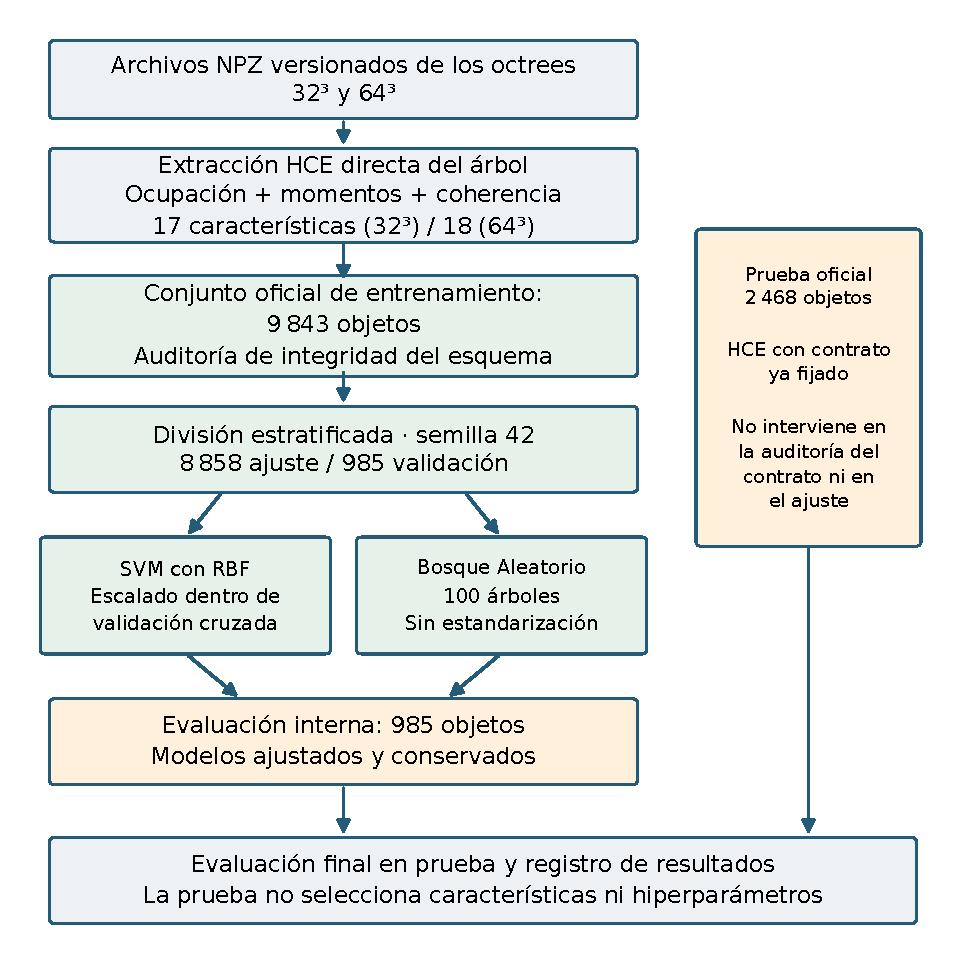
\includegraphics[width=0.96\textwidth,height=0.76\textheight,keepaspectratio]{Figuras/flujo_objetivo2.pdf}
\caption{Flujo metodológico para la extracción de características
    manuales del octree, la preparación de los datos y el entrenamiento
    de los clasificadores tradicionales. El conjunto oficial de prueba
    se mantuvo aislado de la auditoría de características y del ajuste
    de los modelos. Elaboración propia.}
    \label{fig:flujo-objetivo2}
\end{figure}

\subsection{Definición y justificación de las características manuales}
\label{subsec:definicion-caracteristicas-hce}

Se definió un vector de características de dimensión fija a partir de la estructura jerárquica y de las hojas ocupadas del octree. El diseño buscó representar propiedades geométricas relevantes mediante un número reducido de variables interpretables, sin reconstruir una rejilla densa y sin aplicar aprendizaje profundo durante la extracción. Cada objeto quedó descrito mediante tres grupos de características: ocupación jerárquica por nivel, momentos geométricos calculados sobre los centros de las hojas ocupadas y estadísticas de coherencia de las normales.

Sea $L$ la profundidad máxima del octree y sea $N_H$ el número de hojas ocupadas. Todas las hojas consideradas se encuentran en la profundidad $L$, de modo que $L=5$ representa una resolución espacial equivalente de $32^3$ y $L=6$ una de $64^3$. El vector base se denotó mediante $\mathbf h^{(L)}$ y se calculó exclusivamente a partir de los nodos existentes y de la información almacenada en las hojas. Esta formulación conserva el carácter disperso y jerárquico de la representación descrita en la Sección~\ref{subsec:octree-adaptativo}.

\paragraph{Ocupación jerárquica por nivel.}

La primera familia cuantificó la proporción del espacio jerárquico representada por nodos existentes en cada profundidad. En un octree completo, el nivel $d$ puede contener como máximo $8^d$ nodos. Si $N_d$ denota la cantidad de nodos no podados que realmente existen en ese nivel, la Ecuación~\eqref{eq:hce-ocupacion-nivel} define su porcentaje de ocupación.
\begin{equation}
o_d=100\frac{N_d}{8^d},
\qquad d\in\{0,\ldots,L\}.
\label{eq:hce-ocupacion-nivel}
\end{equation}
La cantidad $o_d$ expresa el porcentaje de regiones espaciales activas en la escala asociada con la profundidad $d$. Los niveles poco profundos describen la distribución global del objeto, mientras que los niveles cercanos a $L$ representan detalles espaciales más finos. Esta descripción multiescala aprovecha la organización jerárquica propia de los octrees~\parencite{samet}.

La raíz no se incorporó al vector de entrada de los clasificadores. Para cualquier árbol no vacío se cumple $N_0=1$; por consiguiente, las Ecuaciones~\eqref{eq:hce-raiz-calculo}--\eqref{eq:hce-raiz-constante} muestran que el porcentaje de ocupación de la raíz es constante.
\begin{subequations}\label{eq:hce-ocupacion-raiz}
\begin{align}
o_0&=100\frac{N_0}{8^0}, \label{eq:hce-raiz-calculo} \\
o_0&=100. \label{eq:hce-raiz-constante}
\end{align}
\end{subequations}
Por tanto, $o_0$ no posee capacidad para diferenciar las clases y se conservó únicamente como dato de verificación del extractor. La Ecuación~\eqref{eq:hce-vector-ocupacion} reúne las ocupaciones empleadas como características, desde el primer nivel de subdivisión hasta la profundidad máxima.
\begin{equation}
\mathbf o^{(L)}
=
\begin{bmatrix}
o_1 & o_2 & \cdots & o_L
\end{bmatrix}^{\mathsf T}
\in\mathbb R^L.
\label{eq:hce-vector-ocupacion}
\end{equation}

En el nivel final se cumple $N_L=N_H$ y $8^L=R^3$. La Ecuación~\eqref{eq:hce-ocupacion-hojas} expresa la relación entre la ocupación de ese nivel, el número de hojas y la resolución equivalente.
\begin{equation}
o_L=100\frac{N_H}{R^3}.
\label{eq:hce-ocupacion-hojas}
\end{equation}
Este valor coincide con el porcentaje de celdas ocupadas en la resolución equivalente, aunque se obtuvo directamente del árbol y no mediante la materialización de un tensor denso. Los porcentajes dependen de la escala y de la orientación del objeto respecto de los ejes de subdivisión. La normalización geométrica previa permitió comparar objetos con diferentes tamaños y posiciones, pero no convirtió estos descriptores en invariantes frente a rotaciones.

\paragraph{Momentos geométricos de las hojas ocupadas.}

La segunda familia se calculó sobre los centros de las hojas ocupadas. La Ecuación~\eqref{eq:hce-centros-hojas} establece la notación utilizada para representar el centro de cada hoja.
\begin{equation}
\boldsymbol{\ell}_r=
\begin{bmatrix}
\ell_{r,x} & \ell_{r,y} & \ell_{r,z}
\end{bmatrix}^{\mathsf T},
\qquad r\in\{1,\ldots,N_H\}.
\label{eq:hce-centros-hojas}
\end{equation}
Los vectores $\boldsymbol{\ell}_r$ pertenecen al dominio normalizado $[-1,1]^3$ y se trataron como una nube discreta que describe las regiones del espacio ocupadas por la superficie. Cada hoja recibió el mismo peso, independientemente de la cantidad de puntos superficiales que contuviera. De esta manera, los descriptores caracterizaron la distribución espacial de las regiones ocupadas y no la densidad particular del muestreo dentro de ellas.

Los momentos constituyen una familia clásica de descriptores para caracterizar la distribución espacial de una forma tridimensional~\parencite{sadjadi1980}. En este proyecto se utilizaron estadísticas de primer, segundo y tercer orden por eje, sin construir un conjunto completo de invariantes de momentos. Las Ecuaciones~\eqref{eq:hce-centroide-promedio}--\eqref{eq:hce-centroide-componentes} definen el centroide de los centros de las hojas ocupadas.
\begin{subequations}\label{eq:hce-centroide}
\begin{align}
\boldsymbol\mu&=\frac{1}{N_H}\sum_{r=1}^{N_H}\boldsymbol\ell_r, \label{eq:hce-centroide-promedio} \\
\boldsymbol\mu&=\begin{bmatrix}\mu_x&\mu_y&\mu_z\end{bmatrix}^{\mathsf T}. \label{eq:hce-centroide-componentes}
\end{align}
\end{subequations}
Aunque las mallas fueron centradas antes de construir el octree, $\boldsymbol{\mu}$ no tiene que coincidir exactamente con el origen. La normalización inicial utiliza la media de los vértices, mientras que la Ecuación~\eqref{eq:hce-centroide-promedio} asigna el mismo peso a cada hoja ocupada después de la discretización. Por ello, sus componentes pueden conservar información sobre la distribución asimétrica de la superficie dentro del dominio normalizado.

La dispersión de las hojas a lo largo de cada eje se cuantificó mediante las varianzas poblacionales definidas en la Ecuación~\eqref{eq:hce-varianzas}.
\begin{equation}
v_k
=
\frac{1}{N_H}
\sum_{r=1}^{N_H}
\left(\ell_{r,k}-\mu_k\right)^2,
\qquad k\in\{x,y,z\}.
\label{eq:hce-varianzas}
\end{equation}
Las cantidades $v_x$, $v_y$ y $v_z$ describen la extensión de las hojas respecto del centroide en las tres direcciones cartesianas. Son invariantes frente a una traslación común de los centros, pero dependen de la orientación de la geometría respecto de los ejes del octree. El escalamiento aplicado durante la preparación de las mallas hizo comparables sus magnitudes entre objetos.

La Ecuación~\eqref{eq:hce-dispersion-radial} define la dispersión radial media respecto del centroide.
\begin{equation}
d_{\mathrm{rad}}
=
\frac{1}{N_H}
\sum_{r=1}^{N_H}
\left\|
\boldsymbol{\ell}_r-\boldsymbol{\mu}
\right\|_2.
\label{eq:hce-dispersion-radial}
\end{equation}
Esta medida resume la distancia típica de las regiones ocupadas respecto del centroide sin privilegiar un eje. La norma euclidiana es invariante frente a una rotación común de los centros; sin embargo, el descriptor completo conserva una sensibilidad indirecta a la rotación porque el octree utiliza divisiones alineadas con los ejes y una rotación puede modificar la asignación de la superficie a las hojas.

La asimetría de la distribución espacial se representó mediante el
tercer momento central estandarizado de las coordenadas de los centros
de las hojas. Para estabilizar el cálculo se fijó
$\varepsilon=10^{-12}$. La desviación estándar regularizada y el
coeficiente de asimetría correspondiente a cada eje se definieron
mediante las Ecuaciones~\eqref{eq:hce-desviacion-regularizada} y
\eqref{eq:hce-coeficiente-asimetria}, respectivamente.

\begin{subequations}\label{eq:hce-asimetria}
\begin{align}
\widetilde{\sigma}_k
&=
\sqrt{\max(v_k,\varepsilon)},
\label{eq:hce-desviacion-regularizada}\\
\gamma_k
&=
\frac{
    \displaystyle
    \frac{1}{N_H}
    \sum_{r=1}^{N_H}
    \left(\ell_{r,k}-\mu_k\right)^3
}{
    \widetilde{\sigma}_k^{\,3}+\varepsilon
},
\qquad
k\in\{x,y,z\}.
\label{eq:hce-coeficiente-asimetria}
\end{align}
\end{subequations}

En estas expresiones, $v_k$ es la varianza de las coordenadas de los
centros de las hojas sobre el eje $k$,
$\widetilde{\sigma}_k$ es su desviación estándar regularizada,
$\ell_{r,k}$ es la coordenada de la hoja $r$, $\mu_k$ es la
coordenada correspondiente del centroide y $N_H$ es el número de
hojas ocupadas. El umbral $\varepsilon$ evita operaciones
numéricamente inestables cuando la dispersión sobre un eje es nula o
muy pequeña.

Los coeficientes $\gamma_x$, $\gamma_y$ y $\gamma_z$ describen la
asimetría de la distribución respecto a cada eje cartesiano. Un valor
positivo indica una cola más extendida hacia las coordenadas
positivas, un valor negativo señala una cola más extendida hacia las
coordenadas negativas y un valor cercano a cero corresponde a una
distribución aproximadamente simétrica sobre el eje considerado.
Estas características son adimensionales e invariantes frente a
traslaciones. El tercer momento estandarizado sin regularización
también es invariante frente a factores de escala positivos; sin
embargo, la incorporación del umbral fijo $\varepsilon$ puede alterar
ligeramente esta propiedad cuando la varianza es cercana al límite
numérico. Las características no son invariantes frente a rotaciones,
pues se calcularon separadamente sobre los ejes $x$, $y$ y $z$.

La Ecuación~\eqref{eq:hce-vector-momentos} reúne, en el orden utilizado por el extractor, las diez características correspondientes a los momentos geométricos.
\begin{equation}
\mathbf m=
\begin{bmatrix}
\mu_x &
\mu_y &
\mu_z &
v_x &
v_y &
v_z &
d_{\mathrm{rad}} &
\gamma_x &
\gamma_y &
\gamma_z
\end{bmatrix}^{\mathsf T}
\in\mathbb R^{10}.
\label{eq:hce-vector-momentos}
\end{equation}

\paragraph{Coherencia de las normales.}

La tercera familia de características describió la consistencia de las
orientaciones superficiales dentro de las hojas ocupadas. Sea $m_r$ el
número de muestras asignadas a la hoja $r$ y sean
$\mathbf n_{r,s}$, con $s\in\{1,\ldots,m_r\}$, las normales asociadas
con dichas muestras. El vector normal promedio, antes de su
normalización, se definió mediante la
Ecuación~\eqref{eq:hce-normal-promedio-hoja}, mientras que la
coherencia de la hoja se calculó mediante la
Ecuación~\eqref{eq:hce-coherencia-normal-hoja}.

\begin{subequations}\label{eq:hce-coherencia-hoja}
\begin{align}
\overline{\mathbf n}_r
&=
\frac{1}{m_r}
\sum_{s=1}^{m_r}\mathbf n_{r,s},
\label{eq:hce-normal-promedio-hoja}\\
\rho_r
&=
\left\|
\overline{\mathbf n}_r
\right\|_2.
\label{eq:hce-coherencia-normal-hoja}
\end{align}
\end{subequations}

En estas expresiones, $\overline{\mathbf n}_r$ representa el promedio
vectorial de las normales de las muestras pertenecientes a la hoja
$r$, y $\rho_r$ corresponde a la longitud de dicho vector promedio.
Esta magnitud, denominada longitud resultante media en estadística
direccional, proporciona una medida de la concentración de las
orientaciones~\parencite{mardia1999}. Como cada normal satisface
$\|\mathbf n_{r,s}\|_2\leq 1$, se cumple
$0\leq\rho_r\leq1$.

Un valor de $\rho_r$ cercano a uno indica que las normales asociadas con la hoja presentan orientaciones similares, como puede ocurrir en una región localmente plana o suave. En contraste, un valor cercano a cero indica una baja coherencia direccional producida por la dispersión o cancelación entre orientaciones diferentes. Esta situación puede estar asociada con regiones curvas, aristas, inconsistencias en la orientación de las caras o una combinación de estas condiciones.

La coherencia $\rho_r$ se calculó antes de normalizar el vector promedio $\overline{\mathbf n}_r$. Esta distinción es necesaria porque la norma de una dirección ya normalizada sería unitaria para cualquier hoja con promedio no nulo y, por tanto, no conservaría información sobre la concentración angular de las muestras. El octree almacenó por separado la dirección normalizada, utilizada para representar la orientación superficial, y la coherencia $\rho_r$, empleada posteriormente por el extractor HCE.

La coherencia normal del objeto se resumió mediante la media y la
varianza poblacional de los valores obtenidos sobre las hojas
ocupadas. Estas estadísticas se definieron mediante las
Ecuaciones~\eqref{eq:hce-media-coherencia} y
\eqref{eq:hce-varianza-coherencia}, respectivamente.

\begin{subequations}\label{eq:hce-estadisticas-coherencia}
\begin{align}
\mu_\rho
&=
\frac{1}{N_H}
\sum_{r=1}^{N_H}\rho_r,
\label{eq:hce-media-coherencia}\\
v_\rho
&=
\frac{1}{N_H}
\sum_{r=1}^{N_H}
\left(\rho_r-\mu_\rho\right)^2.
\label{eq:hce-varianza-coherencia}
\end{align}
\end{subequations}

En estas expresiones, $\mu_\rho$ representa la coherencia media de las
hojas ocupadas y resume el grado general de alineación local de las
normales. Por su parte, $v_\rho$ es la varianza poblacional de dichas
coherencias y describe cuánto cambia el grado de alineación entre las
diferentes hojas del objeto. El divisor $N_H$, en lugar de
$N_H-1$, se utilizó porque las hojas ocupadas constituyen la totalidad
de las regiones representadas para cada objeto y no una muestra
seleccionada de ellas.

Cada hoja recibió el mismo peso en las
Ecuaciones~\eqref{eq:hce-media-coherencia} y
\eqref{eq:hce-varianza-coherencia}, independientemente del número de
puntos que contenía. Por consiguiente, estas estadísticas caracterizan
la distribución de las coherencias entre las hojas ocupadas y no un
promedio ponderado sobre todas las muestras superficiales.

La Figura~\ref{fig:familias-descriptores-hce} resume la interpretación geométrica de las tres familias.

\begin{figure}[p]
\centering
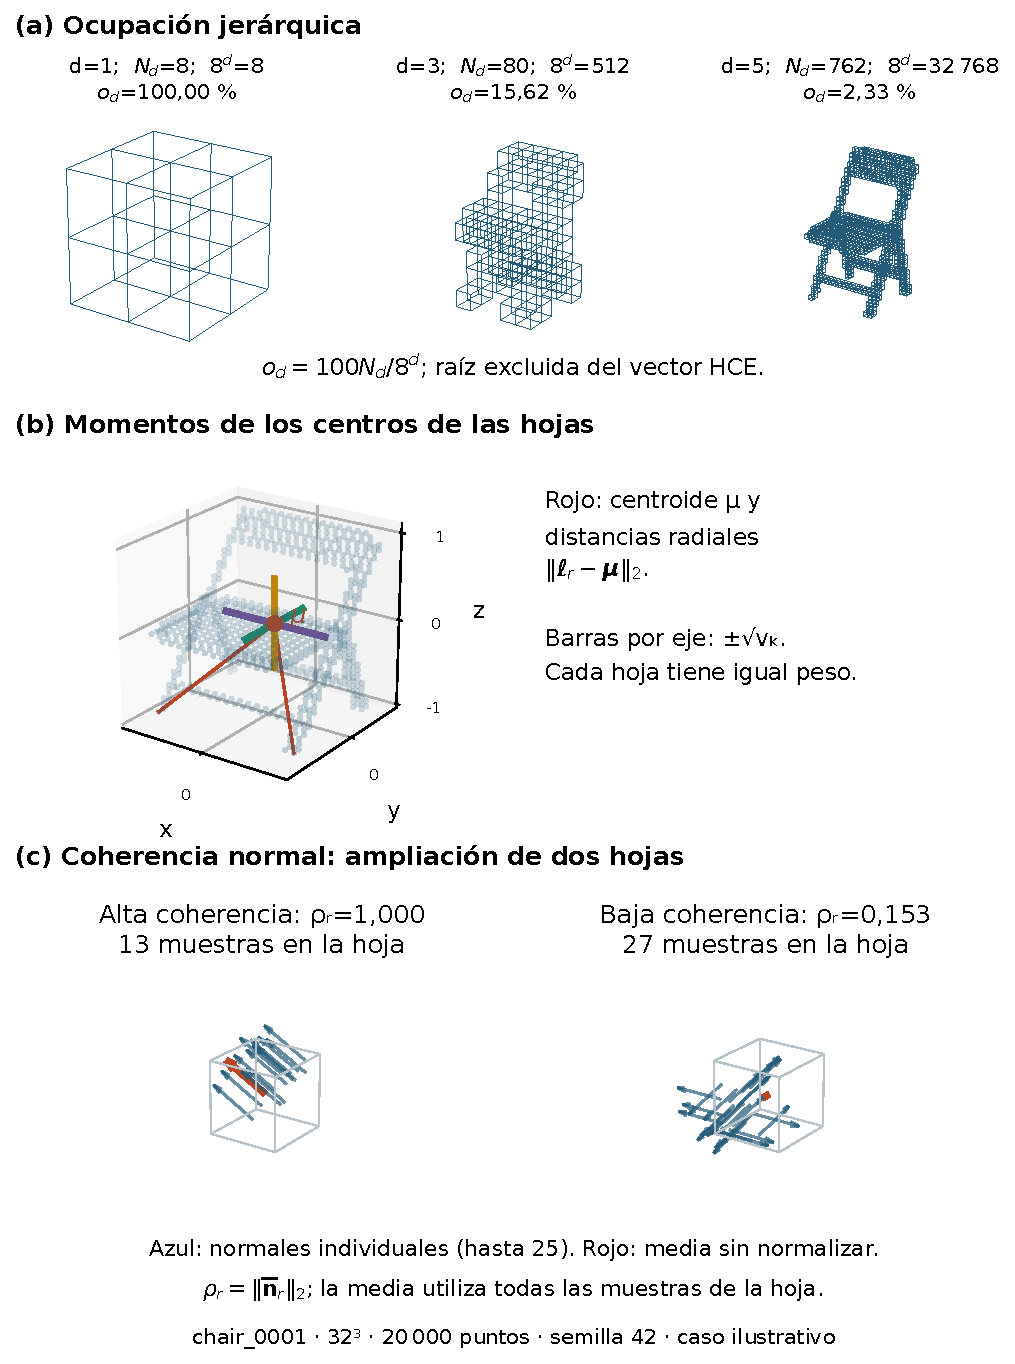
\includegraphics[width=0.96\textwidth,height=0.76\textheight,keepaspectratio]{Figuras/familias_descriptores_hce.pdf}
\caption{Familias de características manuales extraídas del octree:
    (a) ocupación jerárquica por nivel; (b) momentos geométricos
    calculados sobre los centros de las hojas ocupadas; y
    (c) coherencia de las normales dentro de las hojas. La ilustración
    corresponde al procedimiento aplicado directamente sobre la
    representación jerárquica, sin reconstruir una rejilla densa.
    Elaboración propia.}
    \label{fig:familias-descriptores-hce}
\end{figure}

\paragraph{Composición final del vector HCE.}

La Ecuación~\eqref{eq:hce-vector-completo} presenta la concatenación ordenada de las tres familias de descriptores que conforman el vector HCE.
\begin{equation}
\mathbf h^{(L)}
=
\begin{bmatrix}
\underbrace{
o_1,\ldots,o_L
}_{\text{ocupación jerárquica}}
&
\underbrace{
\mu_x,\mu_y,\mu_z,
v_x,v_y,v_z,
d_{\mathrm{rad}},
\gamma_x,\gamma_y,\gamma_z
}_{\text{momentos geométricos}}
&
\underbrace{
\mu_\rho,v_\rho
}_{\text{coherencia de normales}}
\end{bmatrix}^{\mathsf T}.
\label{eq:hce-vector-completo}
\end{equation}

Las Ecuaciones~\eqref{eq:hce-dimension-desglose}--\eqref{eq:hce-dimension-simplificada} establecen la dimensión total del vector en función de la profundidad máxima.
\begin{subequations}\label{eq:hce-dimension}
\begin{align}
\dim(\mathbf h^{(L)})&=L+10+2, \label{eq:hce-dimension-desglose} \\
\dim(\mathbf h^{(L)})&=L+12. \label{eq:hce-dimension-simplificada}
\end{align}
\end{subequations}

La Tabla~\ref{tab:composicion-vector-hce} presenta el orden empleado. Las posiciones se expresan desde uno para facilitar su lectura; la implementación utilizó índices desde cero.

\begin{table}[H]
\centering
\small
\caption{Composición y orden del vector de características HCE.
Elaboración propia.}
\label{tab:composicion-vector-hce}
\begin{tabularx}{\textwidth}{@{}>{\raggedright\arraybackslash\hyphenpenalty=10000}p{3.8cm}X>{\centering\arraybackslash}p{1.7cm}>{\centering\arraybackslash}p{1.7cm}@{}}
\toprule
Familia &
Componentes &
Posiciones en $32^3$ &
Posiciones en $64^3$ \\
\midrule

Ocupación jerárquica &
$o_1,\ldots,o_L$ &
1--5 &
1--6 \\

Momentos geométricos &
$\mu_x,\mu_y,\mu_z$;
$v_x,v_y,v_z$;
$d_{\mathrm{rad}}$;
$\gamma_x,\gamma_y,\gamma_z$ &
6--15 &
7--16 \\

Coherencia de normales &
$\mu_\rho,v_\rho$ &
16--17 &
17--18 \\

\midrule
Total &
$L+12$ componentes &
17 &
18 \\
\bottomrule
\end{tabularx}
\end{table}

La definición del vector base y la exclusión de $o_0$ se establecieron en el extractor antes de aplicar la partición interna: la raíz se excluyó por su constancia analítica, no por un contraste empírico sobre validación o prueba. Las 17 o 18 componentes restantes constituyeron el esquema base para cada resolución. La implementación generó los vectores en formato \texttt{float32}. No se aplicó estandarización durante la extracción; cualquier transformación requerida por un clasificador se incorporó dentro de su procedimiento de ajuste.

\subsection{Partición de los datos y normalización de las características}
\label{subsec:particion-normalizacion-hce}

Los vectores HCE definidos en la Subsección~\ref{subsec:definicion-caracteristicas-hce} se organizaron en matrices independientes para las resoluciones $32^3$ y $64^3$. Para cada resolución $R$, cada fila de la matriz correspondió a un objeto de ModelNet40 y cada columna a una de las características incluidas en el contrato vigente. Por tanto, el conjunto oficial de entrenamiento produjo una matriz $\mathbf X_{\mathrm{train}}^{(R)}\in\mathbb R^{9\,843\times d_R}$ y un vector de etiquetas $\mathbf y_{\mathrm{train}}\in\{0,\ldots,39\}^{9\,843}$, donde $d_{32}=17$ y $d_{64}=18$, de acuerdo con la Ecuación~\eqref{eq:hce-dimension-simplificada}.

Los objetos se recorrieron por categoría y nombre de archivo en un orden determinista. Antes de incorporar un vector a la matriz se verificó que la etiqueta, la partición, la resolución y la profundidad almacenadas en el archivo NPZ coincidieran con los valores esperados. También se comprobó que el número de componentes del vector correspondiera con la dimensión especificada por el contrato de características. Las matrices se almacenaron con tipo \texttt{float32}, mientras que las etiquetas se representaron mediante enteros de tipo \texttt{int64}.

La auditoría de integridad examinó los $9\,843$ objetos del entrenamiento oficial: versiones, metadatos, cantidad de objetos, dimensión, orden de componentes y presencia de valores no finitos. Se registraron adicionalmente estadísticas descriptivas de las columnas. Esta comprobación se distinguió de la definición analítica de los descriptores. El conjunto de prueba no intervino en la auditoría, el escalado ni la selección de modelos.

Los archivos \protect\path{contrato_hce_R32.json} y \protect\path{contrato_hce_R64.json} documentaron el esquema y los índices de entrada. La versión histórica del generador incluía una regla para excluir columnas constantes a partir del entrenamiento oficial completo, antes de reservar la validación. Por ello, no se describió ese mecanismo general como una selección realizada exclusivamente sobre los objetos de ajuste. Se revisaron las exclusiones efectivamente registradas y se comprobó nuevamente la finitud y constancia de las columnas utilizando solo los índices de ajuste reconstruidos. Esta auditoría documental, que no modificó los modelos, se registró en \protect\path{auditoria_documental_contrato_particiones.json}; sus resultados se presentan en el capítulo de resultados. Si una aplicación de esta regla alterase los índices de entrada, la selección tendría que recalcularse sobre el subconjunto de ajuste y los modelos afectados deberían volver a entrenarse.

Una vez finalizada la auditoría, el conjunto oficial de entrenamiento se dividió en un subconjunto de ajuste y un subconjunto de validación. La división se realizó mediante muestreo aleatorio estratificado, reservando el 10\,\% para validación, con barajado habilitado y semilla 42. La estratificación utilizó las etiquetas de las 40 categorías con el fin de conservar, con las aproximaciones enteras necesarias, la distribución de clases del conjunto original.

Como resultado, 8\,858 objetos conformaron el subconjunto de ajuste y 985 objetos el subconjunto de validación. El mismo procedimiento determinista se aplicó a las matrices de ambas resoluciones. El conjunto oficial de prueba, compuesto por 2\,468 objetos, permaneció separado y no participó en la división interna, el cálculo de los parámetros de escalado, la validación cruzada ni la selección de hiperparámetros. La Tabla~\ref{tab:particiones-hce} resume el alcance de cada partición.

\begin{table}[H]
\centering
\small
\caption{Particiones utilizadas para el desarrollo de los clasificadores tradicionales. Elaboración propia.}
\label{tab:particiones-hce}
\begin{tabularx}{\textwidth}{@{}lrrX@{}}
\toprule
Partición & Objetos & Porcentaje & Utilización metodológica \\
\midrule
Entrenamiento oficial completo
& 9\,843
& 100\,\%
& Auditoría de los vectores HCE, generación del contrato de características y origen de la división interna. \\

Ajuste
& 8\,858
& 90\,\% aprox.
& Validación cruzada, estimación de los parámetros de normalización y ajuste de los clasificadores. \\

Validación
& 985
& 10\,\% aprox.
& Evaluación interna de los modelos obtenidos, sin intervenir en el ajuste de sus parámetros. \\

Prueba oficial
& 2\,468
& ---
& Evaluación comparativa final; se mantuvo fuera de la auditoría del contrato, la normalización y la selección de hiperparámetros. \\
\bottomrule
\end{tabularx}
\end{table}

La Figura~\ref{fig:particion-normalizacion-hce} representa el flujo seguido desde los vectores HCE hasta las entradas de los dos clasificadores tradicionales.

\begin{figure}[p]
\centering
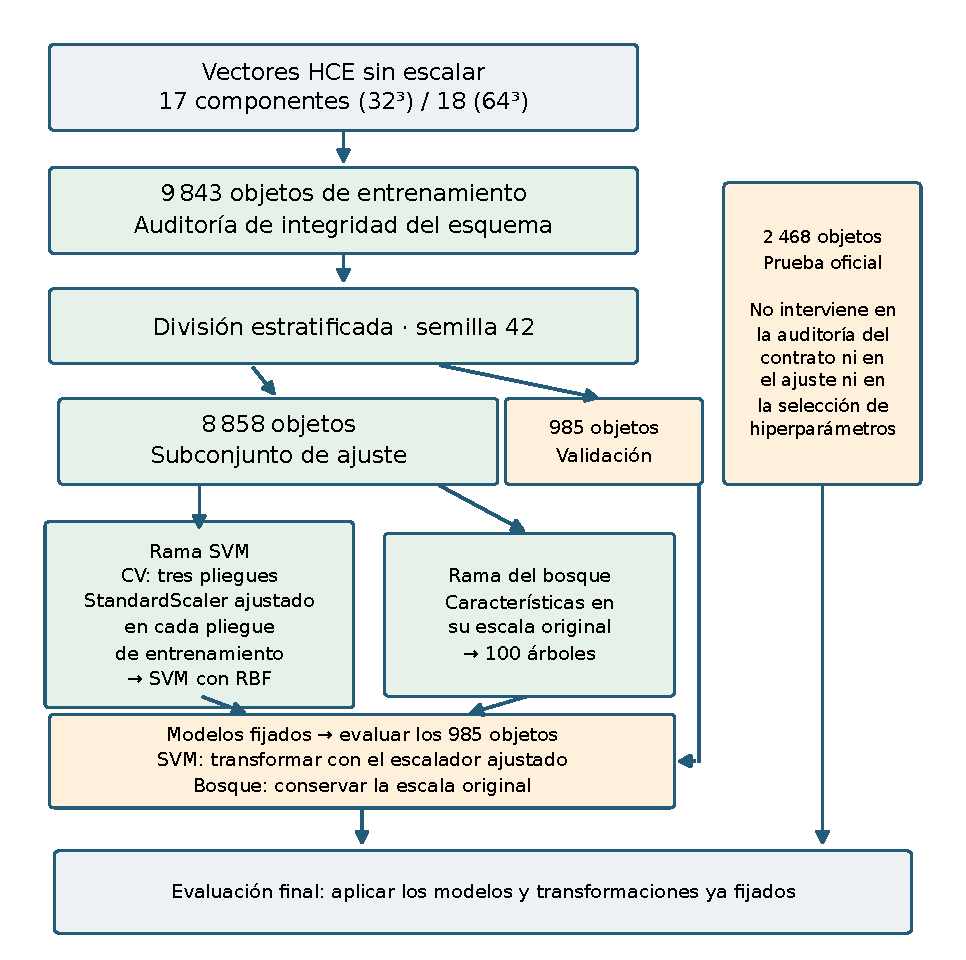
\includegraphics[width=0.96\textwidth,height=0.76\textheight,keepaspectratio]{Figuras/particion_normalizacion_hce.pdf}
\caption{Partición de los vectores HCE y tratamiento aplicado antes del entrenamiento de los clasificadores tradicionales. La estandarización se incorporó exclusivamente en la rama del SVM, mientras que el Bosque Aleatorio recibió las características en su escala original. El conjunto oficial de prueba se mantuvo aislado de las decisiones de ajuste. Elaboración propia.}
\label{fig:particion-normalizacion-hce}
\end{figure}

Las características HCE presentan escalas numéricas diferentes. Por ejemplo, los porcentajes de ocupación se expresan en el intervalo $[0,100]$, mientras que las coordenadas de los centroides, las varianzas geométricas, las asimetrías y las medidas de coherencia poseen intervalos y dispersiones distintos. Estas diferencias afectan especialmente al SVM con kernel RBF, debido a que su medida de similitud depende de las distancias entre los vectores de entrada. Una característica con mayor escala numérica podría dominar dichas distancias aunque no fuera necesariamente más informativa.

Por esta razón, la rama del SVM incorporó una estandarización mediante \texttt{StandardScaler}. Sea $\mathcal I$ el conjunto de índices utilizado para ajustar el transformador y sea $n_{\mathcal I}=|\mathcal I|$ su número de objetos. La media de la característica $k$ sobre dicho conjunto se calculó mediante la Ecuación~\eqref{eq:hce-media-escalado}.

\begin{equation}
\mu_k^{(\mathcal I)}
=
\frac{1}{n_{\mathcal I}}
\sum_{i\in\mathcal I}x_{i,k}.
\label{eq:hce-media-escalado}
\end{equation}

En esta expresión, $x_{i,k}$ es el valor de la característica $k$ para el objeto $i$ y $\mu_k^{(\mathcal I)}$ es su media calculada exclusivamente sobre los objetos pertenecientes al conjunto de ajuste del transformador.

La varianza poblacional utilizada para determinar la dispersión de la característica se definió mediante la Ecuación~\eqref{eq:hce-varianza-escalado}.

\begin{equation}
v_k^{(\mathcal I)}
=
\frac{1}{n_{\mathcal I}}
\sum_{i\in\mathcal I}
\left(
x_{i,k}-\mu_k^{(\mathcal I)}
\right)^2.
\label{eq:hce-varianza-escalado}
\end{equation}

El valor $v_k^{(\mathcal I)}$ representa la varianza de la característica $k$ en el conjunto utilizado para ajustar el escalador. Se empleó el denominador $n_{\mathcal I}$, correspondiente a la varianza poblacional implementada por \texttt{StandardScaler}.

A partir de la media y la varianza anteriores, el valor estandarizado se obtuvo mediante la Ecuación~\eqref{eq:hce-estandarizacion}.

\begin{equation}
z_{i,k}^{(\mathcal I)}
=
\begin{cases}
\dfrac{x_{i,k}-\mu_k^{(\mathcal I)}}
{\sqrt{v_k^{(\mathcal I)}}},
&
v_k^{(\mathcal I)}>0,\\[3mm]
x_{i,k}-\mu_k^{(\mathcal I)},
&
v_k^{(\mathcal I)}=0.
\end{cases}
\label{eq:hce-estandarizacion}
\end{equation}

Aquí, $z_{i,k}^{(\mathcal I)}$ es el valor transformado de la característica $k$ para el objeto $i$. Cuando la varianza es positiva, la transformación centra la característica y la escala por su desviación estándar. Si la varianza es nula, \texttt{StandardScaler} utiliza un factor de escala unitario; por tanto, solo se aplica el centrado. Esta condición describe el comportamiento del transformador cuando una columna resulta constante dentro del subconjunto utilizado para ajustar el escalador.

La estandarización no se ajustó una única vez antes de la búsqueda de hiperparámetros. El escalador y el SVM se integraron en un mismo \texttt{Pipeline}, y este pipeline se entregó al procedimiento de validación cruzada. En cada pliegue, las cantidades $\mu_k^{(\mathcal I)}$ y $v_k^{(\mathcal I)}$ se estimaron exclusivamente con la fracción de entrenamiento de ese pliegue. Posteriormente, esos parámetros se aplicaron a su fracción de validación. Esta organización evitó que las observaciones utilizadas para validar una combinación de hiperparámetros influyeran en las estadísticas de normalización empleadas para entrenarla.

Una vez seleccionada la configuración del SVM, el pipeline completo se reajustó sobre los 8\,858 objetos del subconjunto de ajuste. En este reajuste, el conjunto $\mathcal I$ de las Ecuaciones~\eqref{eq:hce-media-escalado} y \eqref{eq:hce-varianza-escalado} correspondió a la totalidad del subconjunto de ajuste. Los parámetros resultantes se conservaron dentro del modelo y se aplicaron sin modificación a los 985 objetos de validación. Posteriormente, el mismo transformador asociado con el modelo se utilizó para procesar el conjunto oficial de prueba durante la evaluación final.

El Bosque Aleatorio recibió los vectores HCE sin estandarización. Los árboles de decisión seleccionan umbrales sobre cada característica de manera individual; por consiguiente, un cambio lineal positivo en su escala modifica el valor numérico de los umbrales, pero no el orden de las observaciones ni las particiones que pueden producirse. Mantener las características en su escala original evitó incorporar una transformación que no era necesaria para esta familia de modelos.

De este modo, ambos clasificadores utilizaron las mismas características, etiquetas y particiones, pero cada uno recibió el tratamiento numérico apropiado para su mecanismo de aprendizaje. La configuración y el ajuste del SVM con kernel RBF se describen en la Subsección~\ref{subsec:configuracion-svm}, mientras que la configuración del Bosque Aleatorio se presenta en la Subsección~\ref{subsec:configuracion-bosque}.

\subsection{Configuración y ajuste del SVM con kernel RBF}
\label{subsec:configuracion-svm}

El primer clasificador tradicional se implementó mediante una máquina de vectores de soporte, SVM, con kernel de función de base radial, RBF. Las máquinas de vectores de soporte construyen fronteras de decisión de margen máximo y permiten representar separaciones no lineales mediante funciones kernel~\parencite{cortes1995}. En este proyecto, el SVM recibió los vectores HCE estandarizados de acuerdo con el procedimiento descrito en la Subsección~\ref{subsec:particion-normalizacion-hce}.

El entrenamiento se realizó de manera independiente para las resoluciones $32^3$ y $64^3$. En consecuencia, se ajustó un clasificador utilizando vectores de 17 características para $32^3$ y otro utilizando vectores de 18 características para $64^3$. Ambos modelos emplearon las mismas particiones, el mismo espacio de búsqueda de hiperparámetros y el mismo procedimiento de validación cruzada.

Para presentar el funcionamiento del clasificador, considérese inicialmente un problema binario. Sea $\mathbf z_i\in\mathbb R^{d_R}$ el vector HCE estandarizado del objeto $i$ y sea $y_i\in\{-1,+1\}$ su etiqueta dentro de un problema que enfrenta dos clases. El objetivo de la formulación de margen suave se establece mediante la Ecuación~\eqref{eq:svm-objetivo-margen}.

\begin{equation}
\min_{\mathbf w,b,\boldsymbol{\xi}}
\left[
\frac{1}{2}\|\mathbf w\|_2^2
+
C\sum_{i=1}^{n}\xi_i
\right].
\label{eq:svm-objetivo-margen}
\end{equation}

En esta expresión, $\mathbf w$ es el vector normal al hiperplano de separación en el espacio transformado, $b$ es el término independiente, $\xi_i$ es la variable de holgura asociada con el objeto $i$, $n$ es el número de objetos utilizados para el ajuste y $C>0$ es el parámetro de penalización. El primer término favorece un margen amplio, mientras que el segundo penaliza las observaciones que incumplen el margen.

La restricción impuesta a cada observación se expresa mediante la Ecuación~\eqref{eq:svm-restriccion-margen}.

\begin{equation}
y_i
\left[
\mathbf w^{\mathsf T}\phi(\mathbf z_i)+b
\right]
\geq
1-\xi_i,
\qquad
i=1,\ldots,n.
\label{eq:svm-restriccion-margen}
\end{equation}

Aquí, $\phi(\cdot)$ representa una transformación, posiblemente de alta dimensión, inducida por el kernel. Las variables de holgura satisfacen $\xi_i\geq0$. Un valor pequeño de $C$ permite una penalización menor de los incumplimientos del margen y favorece una frontera más regularizada. Por el contrario, un valor elevado incrementa el costo de los errores cometidos sobre las observaciones de ajuste y puede producir una frontera más sensible a estos datos.

No fue necesario construir explícitamente la transformación $\phi(\cdot)$. La similitud entre dos vectores estandarizados se calculó mediante el kernel RBF definido en la Ecuación~\eqref{eq:svm-kernel-rbf}.

\begin{equation}
K_{\gamma}(\mathbf z_i,\mathbf z_j)
=
\exp
\left(
-\gamma
\left\|
\mathbf z_i-\mathbf z_j
\right\|_2^2
\right).
\label{eq:svm-kernel-rbf}
\end{equation}

En esta expresión, $\mathbf z_i$ y $\mathbf z_j$ son dos vectores HCE estandarizados y $\gamma>0$ controla la extensión espacial de la influencia de cada observación. Los valores pequeños de $\gamma$ producen funciones de similitud que decrecen lentamente con la distancia, mientras que los valores elevados concentran la influencia alrededor de cada vector de ajuste.

Una vez resuelto el problema binario, la predicción se determina a partir de los vectores de soporte. La Ecuación~\eqref{eq:svm-decision-binaria} presenta la función de decisión correspondiente.

\begin{equation}
\widehat y(\mathbf z)
=
\operatorname{sign}
\left[
\sum_{i\in\mathcal S}
\alpha_i y_i
K_{\gamma}(\mathbf z_i,\mathbf z)
+b
\right].
\label{eq:svm-decision-binaria}
\end{equation}

El conjunto $\mathcal S$ contiene los índices de los vectores de soporte y $\alpha_i$ representa el coeficiente dual asociado con el objeto $i$. La predicción depende de estos vectores y no de la totalidad de las observaciones utilizadas durante el ajuste.

Debido a que ModelNet40 contiene 40 categorías, la implementación extendió el clasificador binario mediante la estrategia uno contra uno utilizada internamente por \texttt{SVC}. Cada clasificador enfrentó un par de categorías y la decisión multiclase se obtuvo a partir de las decisiones producidas por los clasificadores binarios. Para $K=40$ clases, el número de problemas binarios se calculó mediante la Ecuación~\eqref{eq:svm-numero-pares}.

\begin{equation}
N_{\mathrm{pares}}
=
\frac{K(K-1)}{2}.
\label{eq:svm-numero-pares}
\end{equation}

En esta expresión, $K$ es el número de clases y $N_{\mathrm{pares}}$ es el número de combinaciones diferentes de dos categorías. Por tanto, el ajuste multiclase involucró 780 problemas binarios para cada configuración de hiperparámetros.

Los hiperparámetros $C$ y $\gamma$ se seleccionaron mediante una búsqueda exhaustiva sobre una rejilla discreta. La Tabla~\ref{tab:configuracion-svm} presenta la configuración establecida en la implementación.

\begin{table}[H]
\centering
\small
\caption{Configuración del SVM con kernel RBF y de la búsqueda de hiperparámetros. Elaboración propia.}
\label{tab:configuracion-svm}
\begin{tabularx}{\textwidth}{@{}>{\raggedright\arraybackslash}p{4.1cm}X@{}}
\toprule
Componente & Configuración \\
\midrule
Implementación
& \texttt{SVC} integrado en un \texttt{Pipeline} con \texttt{StandardScaler}. \\

Kernel
& Función de base radial, \texttt{rbf}. \\

Valores de $C$
& $\{0{,}1,\,1,\,10,\,100\}$. \\

Valores de $\gamma$
& $\{\texttt{scale},\,0{,}001,\,0{,}01,\,0{,}1\}$. \\

Combinaciones evaluadas
& 16 combinaciones de $C$ y $\gamma$. \\

Validación cruzada
& Tres pliegues estratificados, con barajado y semilla 42. \\

Criterio de selección
& Mayor exactitud media obtenida en los tres pliegues. \\

Paralelización
& Utilización de los procesadores disponibles mediante \protect\path{n_jobs=-1}. \\

Caché del SVM
& $1\,000$~MB mediante \protect\path{cache_size=1000}. \\

Ponderación de clases
& Sin ponderación adicional; se conservaron los pesos predeterminados. \\
\bottomrule
\end{tabularx}
\end{table}

Cuando $\gamma$ tomó el valor \texttt{scale}, su valor numérico se calculó automáticamente a partir de la matriz estandarizada utilizada para ajustar el SVM. La definición aplicada se presenta en la Ecuación~\eqref{eq:svm-gamma-scale}.

\begin{equation}
\gamma_{\mathrm{scale}}
=
\frac{1}
{d_R\operatorname{Var}
\left(
\mathbf Z_{\mathcal I}
\right)}.
\label{eq:svm-gamma-scale}
\end{equation}

En esta expresión, $d_R$ es la dimensión del vector de características para la resolución $R$ y $\mathbf Z_{\mathcal I}$ es la matriz estandarizada correspondiente al subconjunto utilizado para ajustar el modelo. El operador $\operatorname{Var}(\cdot)$ representa la varianza calculada sobre los valores de esa matriz. Debido a que el escalador se reajustó dentro de cada pliegue, el valor de $\gamma_{\mathrm{scale}}$ también se determinó utilizando únicamente la información disponible en la fracción de entrenamiento correspondiente.

La búsqueda se realizó mediante una validación cruzada estratificada de tres pliegues sobre los 8\,858 objetos del subconjunto de ajuste. Sean $\mathcal F_1$, $\mathcal F_2$ y $\mathcal F_3$ los conjuntos de índices asignados a los tres pliegues. En cada iteración, dos pliegues se utilizaron para ajustar el pipeline y el pliegue restante se utilizó para calcular la exactitud.

Para una combinación determinada de $C$ y $\gamma$, la exactitud obtenida en el pliegue $r$ se calculó mediante la Ecuación~\eqref{eq:svm-exactitud-pliegue}.

\begin{equation}
A_r(C,\gamma)
=
\frac{1}{|\mathcal F_r|}
\sum_{i\in\mathcal F_r}
\mathbf 1
\left[
\widehat y_i^{(-r;C,\gamma)}=y_i
\right].
\label{eq:svm-exactitud-pliegue}
\end{equation}

Aquí, $|\mathcal F_r|$ es el número de objetos del pliegue $r$, $\widehat y_i^{(-r;C,\gamma)}$ es la clase predicha por el modelo ajustado sin utilizar dicho pliegue y $\mathbf 1[\cdot]$ es la función indicadora. La estratificación procuró que cada pliegue mantuviera aproximadamente la distribución de las 40 categorías presente en el subconjunto de ajuste.

La exactitud media de validación cruzada para cada combinación se obtuvo mediante la Ecuación~\eqref{eq:svm-exactitud-media-cv}.

\begin{equation}
\overline{A}_{\mathrm{CV}}(C,\gamma)
=
\frac{1}{3}
\sum_{r=1}^{3}
A_r(C,\gamma).
\label{eq:svm-exactitud-media-cv}
\end{equation}

El valor $\overline{A}_{\mathrm{CV}}(C,\gamma)$ resume el desempeño de una combinación de hiperparámetros en los tres pliegues. Como se evaluaron 16 combinaciones, el procedimiento ejecutó 48 ajustes asociados con la validación cruzada para cada resolución.

La combinación seleccionada se definió mediante la Ecuación~\eqref{eq:svm-seleccion-hiperparametros}.

\begin{equation}
(C^\ast,\gamma^\ast)
=
\underset{
C\in\mathcal C,\,
\gamma\in\mathcal G
}{
\operatorname{arg\,max}
}
\;
\overline{A}_{\mathrm{CV}}(C,\gamma).
\label{eq:svm-seleccion-hiperparametros}
\end{equation}

En esta expresión, $\mathcal C=\{0{,}1;1;10;100\}$ es el conjunto de valores candidatos para $C$ y $\mathcal G=\{\texttt{scale};0{,}001;0{,}01;0{,}1\}$ es el conjunto correspondiente a $\gamma$. Los valores concretos de $C^\ast$ y $\gamma^\ast$ obtenidos para cada resolución se reservan para el capítulo de resultados.

El escalador se mantuvo dentro del pipeline durante todo el procedimiento. Para cada pliegue, sus medias y varianzas se calcularon exclusivamente con los dos pliegues utilizados para el ajuste. La transformación resultante se aplicó después al pliegue retenido. De esta manera, las observaciones empleadas para calcular $A_r(C,\gamma)$ no intervinieron en la estimación de los parámetros de estandarización del modelo evaluado.

Una vez seleccionados $C^\ast$ y $\gamma^\ast$, \texttt{GridSearchCV} reajustó automáticamente el pipeline completo sobre los 8\,858 objetos del subconjunto de ajuste. Este reajuste incluyó nuevamente la estimación de las medias y varianzas del escalador y el entrenamiento del SVM con la configuración seleccionada. Por tanto, el modelo obtenido conservó dentro del mismo objeto computacional tanto el transformador como el clasificador.

La Figura~\ref{fig:ajuste-svm-rbf} resume el procedimiento de búsqueda y reajuste del SVM.

\begin{figure}[p]
\centering
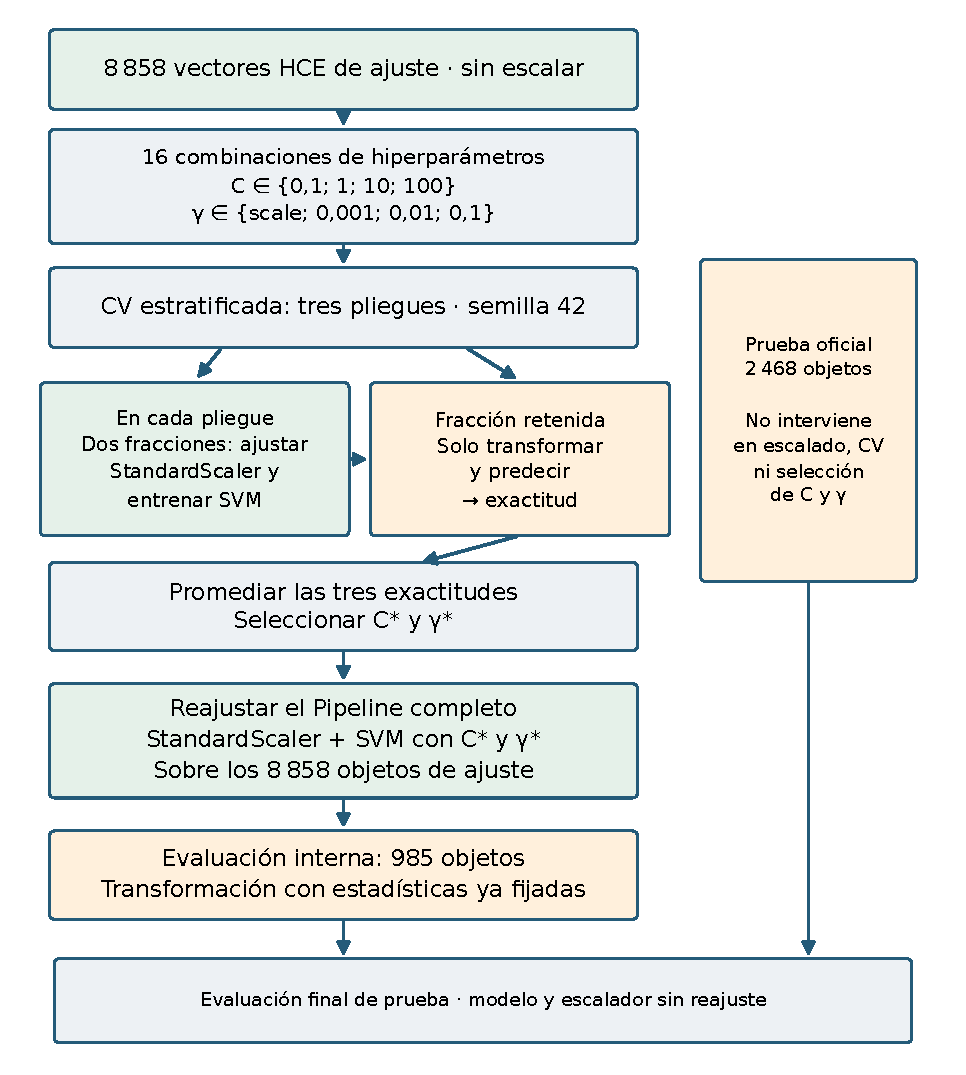
\includegraphics[width=0.96\textwidth,height=0.76\textheight,keepaspectratio]{Figuras/ajuste_svm_rbf.pdf}
\caption{Procedimiento de selección de hiperparámetros y ajuste del SVM con kernel RBF. La estandarización se integró en el pipeline de validación cruzada para impedir que los pliegues retenidos influyeran en sus parámetros. Después de seleccionar la mejor configuración, el pipeline se reajustó sobre el subconjunto completo de ajuste. Elaboración propia.}
\label{fig:ajuste-svm-rbf}
\end{figure}

El modelo reajustado se aplicó posteriormente a los 985 objetos del subconjunto de validación, sin volver a estimar los parámetros del escalador ni modificar $C^\ast$ o $\gamma^\ast$. La exactitud de validación se definió mediante la Ecuación~\eqref{eq:svm-exactitud-validacion}.

\begin{equation}
A_{\mathrm{val}}
=
\frac{1}{N_{\mathrm{val}}}
\sum_{i=1}^{N_{\mathrm{val}}}
\mathbf 1
\left[
\widehat y_i=y_i
\right].
\label{eq:svm-exactitud-validacion}
\end{equation}

En esta expresión, $N_{\mathrm{val}}=985$, $y_i$ es la categoría verdadera del objeto de validación y $\widehat y_i$ es la categoría predicha por el pipeline reajustado. Esta medición permitió verificar el comportamiento interno del modelo sin utilizar los 2\,468 objetos del conjunto oficial de prueba. Los valores seleccionados de los hiperparámetros, la exactitud alcanzada y el tiempo requerido por la búsqueda se presentan posteriormente como resultados experimentales.

\subsection{Configuración y entrenamiento del Bosque Aleatorio}
\label{subsec:configuracion-bosque}

El segundo clasificador tradicional se implementó mediante un Bosque Aleatorio, \textit{Random Forest}, un método de ensamble que combina múltiples árboles de decisión construidos a partir de muestras y subconjuntos de características seleccionados aleatoriamente~\parencite{breiman2001}. Esta combinación reduce la correlación entre los árboles y busca mejorar la capacidad de generalización respecto de un único árbol de decisión.

El entrenamiento se realizó de manera independiente para las resoluciones $32^3$ y $64^3$. Cada modelo recibió los vectores HCE correspondientes a su resolución: 17 características para $32^3$ y 18 características para $64^3$. En ambos casos se emplearon los mismos 8\,858 objetos del subconjunto de ajuste definido en la Subsección~\ref{subsec:particion-normalizacion-hce}.

A diferencia del SVM con kernel RBF, el Bosque Aleatorio recibió las características en su escala original. Los árboles de decisión establecen sus separaciones mediante comparaciones de la forma $x_k\leq\tau$, donde $x_k$ es el valor de una característica y $\tau$ un umbral. Una transformación lineal positiva de una característica modifica el valor numérico del umbral, pero conserva el orden de las observaciones y, por tanto, las particiones que pueden construirse. En consecuencia, no se incorporó un escalador en esta rama del procedimiento.

Se construyó un ensamble de $B=100$ árboles. Para cada árbol se generó, de manera predeterminada, una muestra \textit{bootstrap} del mismo tamaño que el subconjunto de ajuste. Esta muestra se obtuvo mediante extracciones con reemplazo, por lo que un objeto pudo aparecer varias veces en el entrenamiento de un árbol y otros objetos pudieron quedar fuera de su muestra particular.

En cada nodo se evaluó únicamente un subconjunto aleatorio de las características disponibles. Se conservó el valor predeterminado \protect\path{max_features=sqrt}, correspondiente aproximadamente a $\sqrt{d_R}$ características candidatas por división. Puesto que $d_{32}=17$ y $d_{64}=18$, en ambas resoluciones se consideraron cuatro características candidatas en cada nodo. La selección se realizó nuevamente en cada división y de manera independiente entre los árboles.

El criterio utilizado para evaluar la pureza de un nodo fue la impureza de Gini. Sea $\mathcal S_\nu$ el conjunto de observaciones que alcanza el nodo $\nu$. La impureza de ese nodo se definió mediante la Ecuación~\eqref{eq:rf-gini}.

\begin{equation}
G(\mathcal S_\nu)
=
1-
\sum_{c=0}^{K-1}
p_{c,\nu}^{\,2}.
\label{eq:rf-gini}
\end{equation}

En esta expresión, $K=40$ es el número de categorías de ModelNet40 y $p_{c,\nu}$ es la proporción de observaciones de la clase $c$ presentes en el nodo $\nu$, con $c\in\{0,\ldots,K-1\}$, de acuerdo con la indexación de las etiquetas utilizada en la implementación. La impureza es igual a cero cuando todas las observaciones del nodo pertenecen a una misma clase y aumenta cuando las observaciones se distribuyen entre diferentes categorías.

Para una característica candidata $k$ y un umbral $\tau$, el conjunto $\mathcal S_\nu$ se dividió en un subconjunto izquierdo $\mathcal S_{\nu,L}$ y un subconjunto derecho $\mathcal S_{\nu,R}$. La impureza ponderada producida por esa división se calculó mediante la Ecuación~\eqref{eq:rf-impureza-division}.

\begin{equation}
G_{\mathrm{div}}
\left(
\mathcal S_\nu;k,\tau
\right)
=
\frac{|\mathcal S_{\nu,L}|}{|\mathcal S_\nu|}
G(\mathcal S_{\nu,L})
+
\frac{|\mathcal S_{\nu,R}|}{|\mathcal S_\nu|}
G(\mathcal S_{\nu,R}).
\label{eq:rf-impureza-division}
\end{equation}

Aquí, $|\mathcal S_\nu|$ es el número de observaciones que alcanza el nodo padre, mientras que $|\mathcal S_{\nu,L}|$ y $|\mathcal S_{\nu,R}|$ son los tamaños de los nodos hijos. Para cada nodo se seleccionó la característica y el umbral que produjeron la menor impureza ponderada entre las divisiones candidatas.

La reducción de impureza conseguida por una división se definió mediante la Ecuación~\eqref{eq:rf-reduccion-impureza}.

\begin{equation}
\Delta G_\nu
=
G(\mathcal S_\nu)
-
G_{\mathrm{div}}
\left(
\mathcal S_\nu;k^\ast,\tau^\ast
\right).
\label{eq:rf-reduccion-impureza}
\end{equation}

Los símbolos $k^\ast$ y $\tau^\ast$ representan, respectivamente, la característica y el umbral seleccionados para el nodo $\nu$. Los valores positivos de $\Delta G_\nu$ indican que la división incrementó la pureza de los nodos resultantes.

No se impuso una profundidad máxima a los árboles, pues se configuró \protect\path{max_depth=None}. En consecuencia, cada árbol pudo continuar expandiéndose hasta alcanzar hojas puras, nodos que no admitieran una división válida o nodos con un número de observaciones inferior al requerido para subdividirse. Se conservaron los valores predeterminados de dos observaciones para dividir un nodo y una observación como tamaño mínimo de una hoja.

Para clasificar un nuevo vector $\mathbf x$, cada árbol lo condujo desde la raíz hasta una hoja terminal. La probabilidad asignada por el árbol $b$ a la clase $c$ se calculó mediante la Ecuación~\eqref{eq:rf-probabilidad-arbol}.

\begin{equation}
\widehat p_c^{(b)}(\mathbf x)
=
\frac{
N_{\ell_b(\mathbf x),c}^{(b)}
}{
N_{\ell_b(\mathbf x)}^{(b)}
}.
\label{eq:rf-probabilidad-arbol}
\end{equation}

En esta expresión, $\ell_b(\mathbf x)$ identifica la hoja alcanzada por $\mathbf x$ en el árbol $b$, $N_{\ell_b(\mathbf x),c}^{(b)}$ es el número de observaciones de la clase $c$ presentes en esa hoja y $N_{\ell_b(\mathbf x)}^{(b)}$ es el número total de observaciones de la hoja.

La probabilidad estimada por el bosque para la clase $c$ se obtuvo promediando las probabilidades producidas por los 100 árboles. Esta agregación se define mediante la Ecuación~\eqref{eq:rf-probabilidad-bosque}.

\begin{equation}
\widehat p_c(\mathbf x)
=
\frac{1}{B}
\sum_{b=1}^{B}
\widehat p_c^{(b)}(\mathbf x).
\label{eq:rf-probabilidad-bosque}
\end{equation}

Aquí, $B=100$ es el número total de árboles y $\widehat p_c(\mathbf x)$ es la probabilidad promedio asignada a la clase $c$. La categoría predicha se seleccionó mediante la Ecuación~\eqref{eq:rf-prediccion}.

\begin{equation}
\widehat y(\mathbf x)
=
\underset{c\in\{0,\ldots,39\}}
{\operatorname{arg\,max}}
\;
\widehat p_c(\mathbf x).
\label{eq:rf-prediccion}
\end{equation}

El valor $\widehat y(\mathbf x)$ corresponde a la categoría con mayor probabilidad promedio en el ensamble. Esta regla permite combinar las decisiones de árboles entrenados con diferentes muestras \textit{bootstrap} y diferentes subconjuntos de características.

La Tabla~\ref{tab:configuracion-rf} reúne los parámetros utilizados. Los parámetros no suministrados explícitamente al constructor conservaron los valores predeterminados de la versión de \texttt{scikit-learn} registrada en el entorno computacional.

\begin{table}[H]
\centering
\small
\caption{Configuración utilizada para el entrenamiento del Bosque Aleatorio. Elaboración propia.}
\label{tab:configuracion-rf}
\begin{tabularx}{\textwidth}{@{}p{4.3cm}X@{}}
\toprule
Parámetro & Valor o condición \\
\midrule
Número de árboles
& 100. \\

Criterio de división
& Impureza de Gini. \\

Profundidad máxima
& Sin límite explícito, \protect\path{max_depth=None}. \\

Características candidatas
& $\sqrt{d_R}$ por nodo; cuatro características para ambas resoluciones. \\

Muestreo de objetos
& Muestras \textit{bootstrap} con reemplazo. \\

Mínimo para dividir un nodo
& Dos observaciones. \\

Mínimo por hoja
& Una observación. \\

Ponderación de clases
& Sin ponderación adicional, \protect\path{class_weight=None}. \\

Semilla
& 42. \\

Paralelización
& Todos los procesadores disponibles mediante \protect\path{n_jobs=-1}. \\

Normalización de entrada
& No se aplicó estandarización. \\
\bottomrule
\end{tabularx}
\end{table}

No se realizó una búsqueda de hiperparámetros para el Bosque Aleatorio. La configuración de la Tabla~\ref{tab:configuracion-rf} se estableció como una línea base fija para las dos resoluciones. Por tanto, la exactitud obtenida sobre el subconjunto de validación no corresponde al máximo de una rejilla de configuraciones, sino al desempeño de este clasificador bajo los parámetros preestablecidos.

La semilla 42 controló tanto la obtención de las muestras \textit{bootstrap} como la selección aleatoria de características en los nodos. Esta configuración permitió reproducir la construcción del ensamble al mantener constantes los datos, el orden de entrada y el entorno de ejecución. El parámetro \protect\path{n_jobs=-1} habilitó el uso de todos los núcleos de CPU disponibles; la tarjeta gráfica no intervino en este entrenamiento.

La Figura~\ref{fig:bosque-aleatorio-hce} resume la construcción y la agregación de los árboles.

\begin{figure}[p]
\centering
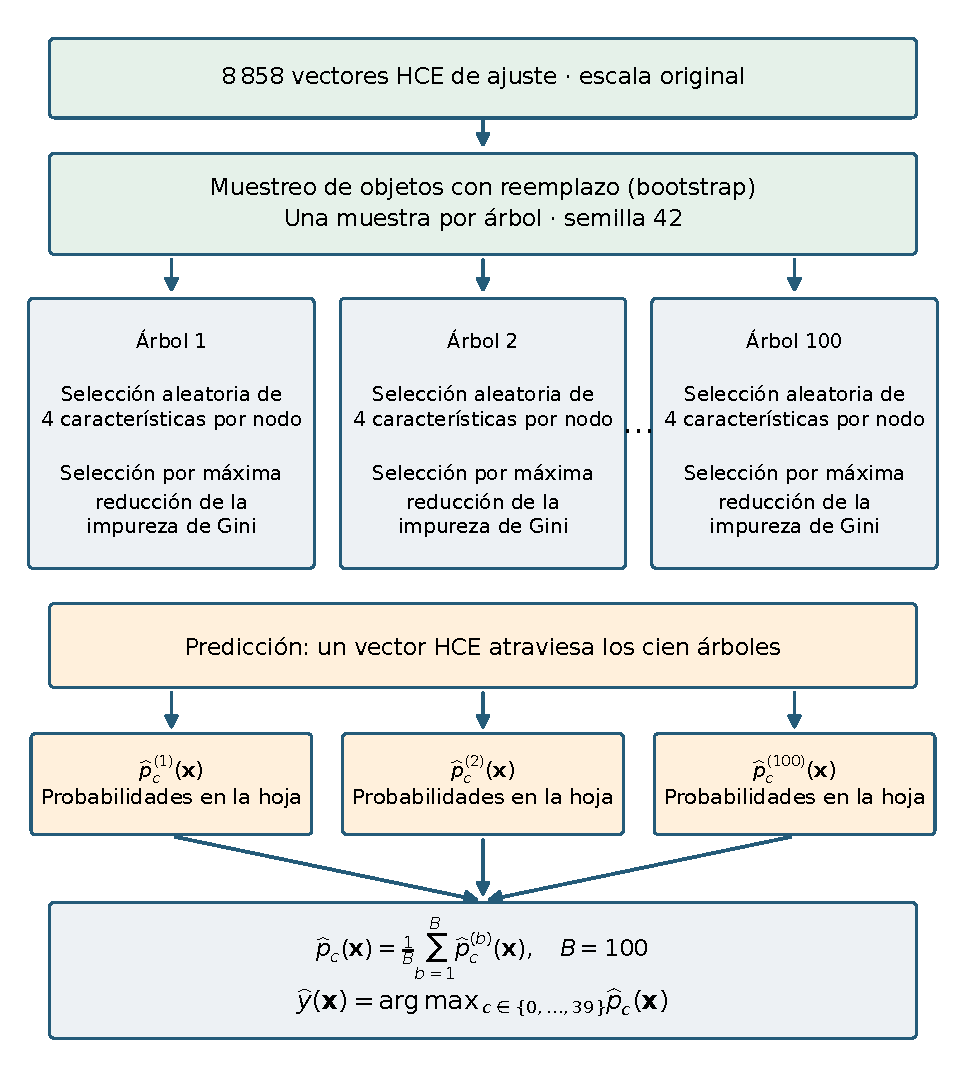
\includegraphics[width=0.96\textwidth,height=0.76\textheight,keepaspectratio]{Figuras/bosque_aleatorio_hce.pdf}
\caption{Construcción del Bosque Aleatorio a partir de los vectores HCE. Cada árbol se entrenó con una muestra \textit{bootstrap} y evaluó subconjuntos aleatorios de características en sus nodos. La predicción final se obtuvo promediando las probabilidades de clase producidas por los 100 árboles. Elaboración propia.}
\label{fig:bosque-aleatorio-hce}
\end{figure}

Después del entrenamiento, el modelo se aplicó a los 985 objetos del subconjunto de validación. La exactitud se calculó con el mismo criterio establecido en la Ecuación~\eqref{eq:svm-exactitud-validacion}. Este subconjunto no intervino en la construcción de los árboles, la generación de las muestras \textit{bootstrap} ni la selección de las divisiones.

El intervalo de entrenamiento se midió desde antes de crear y ajustar el clasificador hasta el retorno de la operación \texttt{fit}. Por tanto, incluyó la construcción de los 100 árboles, pero excluyó la predicción sobre el subconjunto de validación, el cálculo de las métricas y la escritura del modelo en el sistema de archivos.

Además de las predicciones, se conservaron las importancias de las características calculadas mediante la reducción media de impureza. Para cada característica se acumularon las reducciones de Gini producidas por los nodos que la utilizaron, ponderadas por el número de observaciones que alcanzó cada nodo y agregadas sobre los 100 árboles. Las importancias se normalizaron para que su suma fuera igual a uno. Estos valores se registraron como información auxiliar para analizar la contribución relativa de las características HCE, sin interpretarlos como efectos causales.

Los valores de exactitud, tiempo de entrenamiento e importancia de las características no se incorporaron en esta subsección, pues corresponden a los resultados experimentales. El procedimiento de validación interna y la persistencia de los modelos se describen en la Subsección~\ref{subsec:validacion-persistencia-tradicional}.


\subsection{Validación interna, evaluación y persistencia de los modelos}
\label{subsec:validacion-persistencia-tradicional}

La validación interna y la evaluación final se realizaron por separado para cada resolución y clasificador. Después del ajuste sobre los $8\,858$ objetos, los modelos se aplicaron a los 985 objetos del subconjunto de validación y se registró su exactitud mediante el criterio de la Ecuación~\eqref{eq:svm-exactitud-validacion}. En el SVM, esta evaluación fue posterior a la selección de hiperparámetros mediante validación cruzada dentro del subconjunto de ajuste. En el Bosque Aleatorio, se evaluó la configuración fija descrita en la Subsección~\ref{subsec:configuracion-bosque}. Los 985 objetos no se utilizaron para estimar el escalador, ajustar los clasificadores ni construir los árboles.

La evaluación final utilizó los $2\,468$ objetos de la partición oficial de prueba. Se conservaron el orden y la dimensión de las características establecidos por el contrato correspondiente a cada resolución. El SVM recibió los vectores sin escalar como entrada a su \texttt{Pipeline}, que aplicó el \texttt{StandardScaler} ya ajustado antes de predecir. El Bosque Aleatorio recibió las características en su escala original. No se efectuó un reajuste adicional sobre los $9\,843$ objetos de entrenamiento antes de evaluar en prueba: se emplearon los modelos ajustados con los $8\,858$ objetos. El conjunto de prueba no intervino en la selección del contrato, en la estimación de las estadísticas del escalador ni en la búsqueda de hiperparámetros.

\paragraph{Métricas de clasificación.}

Para cada modelo se obtuvo un vector de predicciones y se calculó la exactitud global. También se construyó una matriz de confusión de $40\times40$, manteniendo el orden de las categorías utilizado por la implementación. La Ecuación~\eqref{eq:hce-matriz-confusion} define los conteos de esta matriz.
\begin{equation}
M_{c,j}=\sum_{i=1}^{n_{\mathrm{test}}}
\mathbb{I}\!\left(y_i=c\;\land\;\widehat y_i=j\right),
\qquad c,j\in\{0,\ldots,39\}.
\label{eq:hce-matriz-confusion}
\end{equation}
En esta expresión, $n_{\mathrm{test}}=2\,468$ es el número de objetos de prueba, $y_i$ es la clase real del objeto $i$, $\widehat y_i$ su clase predicha y $\mathbb{I}$ vale uno cuando se cumple la condición indicada y cero en caso contrario. Las filas de $M$ corresponden a las clases reales y las columnas a las predicciones. Se conservaron conteos absolutos; cualquier normalización de una matriz para su visualización pertenece a la presentación de resultados y no modifica estos registros.

A partir de esos conteos se definieron los verdaderos positivos, falsos positivos y falsos negativos de cada clase mediante las Ecuaciones~\eqref{eq:hce-verdaderos-positivos}--\eqref{eq:hce-falsos-negativos}.
\begin{subequations}\label{eq:hce-conteos-clase}
\begin{align}
\mathrm{VP}_c &= M_{c,c}, \label{eq:hce-verdaderos-positivos} \\
\mathrm{FP}_c &= \sum_{j\ne c}M_{j,c}, \label{eq:hce-falsos-positivos} \\
\mathrm{FN}_c &= \sum_{j\ne c}M_{c,j}. \label{eq:hce-falsos-negativos}
\end{align}
\end{subequations}
Aquí, $j$ recorre las restantes categorías; $\mathrm{VP}_c$ cuenta los aciertos de la clase $c$, $\mathrm{FP}_c$ las asignaciones incorrectas a esa clase y $\mathrm{FN}_c$ sus objetos asignados a otras clases. Estos conteos permiten calcular las métricas por categoría definidas en las Ecuaciones~\eqref{eq:hce-precision-clase}--\eqref{eq:hce-f1-clase}.
\begin{subequations}\label{eq:hce-metricas-clase}
\begin{align}
P_c &= \frac{\mathrm{VP}_c}{\mathrm{VP}_c+\mathrm{FP}_c}, \label{eq:hce-precision-clase} \\
S_c &= \frac{\mathrm{VP}_c}{\mathrm{VP}_c+\mathrm{FN}_c}, \label{eq:hce-sensibilidad-clase} \\
F_{1,c} &= \frac{2P_cS_c}{P_c+S_c}. \label{eq:hce-f1-clase}
\end{align}
\end{subequations}
Los símbolos $P_c$, $S_c$ y $F_{1,c}$ representan, respectivamente, la precisión, la sensibilidad y la media armónica de ambas para la clase $c$. Se utilizó \protect\path{classification_report} con \protect\path{zero_division=0}, por lo que las métricas cuyo denominador fue nulo se registraron como cero. El informe incluyó el soporte de cada clase, definido como su número de objetos reales, y los promedios macro y ponderado de las métricas. El promedio macro asigna igual peso a las 40 clases; el ponderado utiliza sus respectivos soportes. Todas estas métricas se almacenaron como proporciones adimensionales; su expresión porcentual se reservó para la presentación de resultados.

\paragraph{Medición de inferencia y tamaño de los modelos.}

El tiempo de inferencia se midió mediante \texttt{time.time}, inmediatamente antes y después de una llamada a \texttt{predict} sobre la matriz completa de prueba. Para el SVM, la llamada incluyó la transformación de las características mediante el escalador del \texttt{Pipeline}. Para el Bosque Aleatorio, correspondió a la predicción del ensamble. En ambos casos quedaron fuera del intervalo la lectura de los octrees, la extracción HCE, el cálculo de las métricas de clasificación y la escritura de los resultados.

El promedio por objeto se calculó mediante la Ecuación~\eqref{eq:hce-tiempo-inferencia}.
\begin{equation}
\overline t_{\mathrm{inf}}
=\frac{1\,000\,t_{\mathrm{inf}}}{n_{\mathrm{test}}}\;\mathrm{ms}.
\label{eq:hce-tiempo-inferencia}
\end{equation}
Aquí, $t_{\mathrm{inf}}$ es el valor numérico del intervalo total expresado en segundos y $n_{\mathrm{test}}$ es el número de objetos evaluados. El factor $1\,000$ convierte segundos en milisegundos. Este cociente representa el tiempo medio por objeto de una predicción por lote; no corresponde a una medición independiente de latencia para cada objeto. La implementación registró una llamada de predicción por clasificador y resolución, sin repeticiones temporales adicionales en este procedimiento.

Después de guardar los modelos, su tamaño se obtuvo consultando los bytes del archivo cerrado y dividiendo entre $10^6$ para expresarlo en MB decimales. Esta magnitud describe almacenamiento en disco, no memoria residente ni pico de memoria durante entrenamiento o inferencia. Los tiempos de ajuste conservaron el alcance de las subsecciones anteriores: búsqueda y reajuste del SVM, por una parte, y construcción del bosque con su configuración fija, por otra.

\paragraph{Persistencia y trazabilidad.}

Se utilizó \texttt{joblib.dump} para conservar un modelo por clasificador y resolución. El archivo del SVM incluyó el \texttt{Pipeline} completo, de modo que el escalador y el clasificador permanecieron asociados. El archivo del Bosque Aleatorio conservó el estimador ajustado. También se guardó un archivo NPZ con las matrices HCE del entrenamiento oficial y de prueba, sus etiquetas, los nombres ordenados de las características y la versión del contrato. Este archivo contiene características extraídas, no un nuevo conjunto de datos independiente de las particiones originales.

La Tabla~\ref{tab:hce-archivos-persistencia} resume los archivos producidos. En sus nombres, \texttt{R32} o \texttt{R64} identifica la resolución de la ejecución; los directorios de salida se establecieron mediante los parámetros del programa.
\begin{table}[htbp]
\centering\small
\caption{Archivos de características, modelos y evaluación del enfoque HCE. Elaboración propia.}
\label{tab:hce-archivos-persistencia}
\begin{tabularx}{\textwidth}{@{}>{\raggedright\arraybackslash}p{5.4cm}>{\raggedright\arraybackslash}X@{}}
\toprule
Archivos generados & Contenido \\
\midrule
\protect\path{hce_features_R32.npz} \newline \protect\path{hce_features_R64.npz} & Características, etiquetas, orden de columnas y versión del contrato. \\
\protect\path{hce_svm_R32.joblib} \newline \protect\path{hce_svm_R64.joblib} & Escalador y SVM ajustados dentro de un mismo \texttt{Pipeline}. \\
\protect\path{hce_rf_R32.joblib} \newline \protect\path{hce_rf_R64.joblib} & Bosque Aleatorio ajustado. \\
\protect\path{resumen_hce_R32.json} \newline \protect\path{resumen_hce_R64.json} & Configuración, métricas, matrices de confusión e importancias del bosque. \\
\protect\path{validacion_entrenamientos_hce.json} & Informe de consistencia de los resúmenes de ambas resoluciones. \\
\bottomrule
\end{tabularx}
\end{table}

Los resúmenes JSON registraron la versión del esquema, la resolución, la profundidad, el contrato utilizado, las características excluidas y el orden de entrada al modelo. Asimismo, incluyeron los tamaños de las particiones, la semilla, los hiperparámetros seleccionados del SVM, la configuración principal del bosque, las exactitudes de validación y prueba, los tiempos, los tamaños de los modelos, los informes por clase y las matrices de confusión. Las importancias del bosque se asociaron con los nombres de las características y se ordenaron de mayor a menor valor. La escritura de los resúmenes rechazó valores no finitos mediante \protect\path{allow_nan=False}.

La consistencia de los resúmenes se verificó mediante \protect\path{validar_resultados_hce.py}, contrastando los archivos de ambas resoluciones con sus contratos. Se comprobaron los esquemas, dimensiones, orden de características, conteos de las particiones y rangos de las métricas. Además, se contrastaron la exactitud con la diagonal de la matriz de confusión, los soportes por clase con las sumas de sus filas y el tiempo medio de inferencia con el tiempo total y el número de objetos. Para el bosque se verificaron los nombres, la cantidad y la normalización de las importancias; para el SVM, la pertenencia de los hiperparámetros a la rejilla autorizada. El informe consolidado registró las incidencias y el estado de validación de cada resolución.

Esta comprobación evaluó la consistencia de los registros experimentales; no sustituyó una nueva ejecución del entrenamiento ni una prueba de recarga y equivalencia de los archivos \texttt{joblib}. Los valores obtenidos y las comparaciones entre clasificadores y resoluciones se presentan en el capítulo de resultados. La descripción inicial de este procedimiento se contrastó con la versión \texttt{3e596ce}. La revisión final incorporó la comparación y reevaluación disponibles en \texttt{64b8835}, manteniendo diferenciadas la auditoría de resúmenes y la ejecución de los modelos persistidos.


\section{Modelo profundo Net5}
\label{sec:net5-metodologia}

Esta sección desarrolla el tercer objetivo específico: implementar, entrenar y configurar una red profunda basada en octrees de tipo Net5 bajo las mismas particiones de datos y resoluciones equivalentes de $32^3$ y $64^3$. Para estudiar el aprendizaje de características sobre las representaciones jerárquicas se implementó una adaptación de Net5 para las 40 categorías de ModelNet40. Se tomó como referencia la arquitectura de clasificación de capacidad fija descrita en el material suplementario de OctNet, cuya representación híbrida combina una rejilla regular con octrees de profundidad limitada \parencite{riegler2017}. La adaptación del proyecto incorporó cuatro canales de entrada y una salida de 40 clases. Se mantuvo la misma cantidad de parámetros entrenables al cambiar de resolución, con el fin de separar el efecto de la resolución del aumento de capacidad del modelo.

El procedimiento comprendió la lectura de los octrees serializados, su conversión a la estructura utilizada por las operaciones de la red, el entrenamiento supervisado y la selección del estado con mayor exactitud de validación. Esta sección describe la implementación nativa y la configuración de las ejecuciones completas registradas con el identificador de versión \texttt{8164428}. Las exactitudes obtenidas, las curvas de aprendizaje y las comparaciones cuantitativas se reservan para el capítulo de resultados.

\subsection{Representación de entrada}
\label{subsec:net5-entrada}

Se utilizaron los archivos NPZ generados por el procesamiento geométrico descrito previamente, con resolución equivalente $R=32$ o $R=64$ y profundidad máxima global $L=5$ o $L=6$, respectivamente. Para cada objeto se reconstruyó el árbol a partir de sus profundidades, máscaras de hijos, normales y coherencias. Durante la carga se verificó que la resolución declarada coincidiera con la de la ejecución y que la etiqueta almacenada correspondiera a la categoría del objeto. No se efectuó un nuevo muestreo de la malla durante el entrenamiento.

El árbol global se convirtió en una rejilla de octrees de profundidad local máxima tres, siguiendo el principio de representación híbrida de OctNet \parencite{riegler2017}. Cada árbol local cubrió un bloque de ocho celdas finas por eje. Por tanto, la rejilla de raíces locales contó con cuatro árboles por eje para $R=32$ y ocho para $R=64$. La profundidad local se distingue del nivel global $L$: la raíz del octree geométrico original conserva la convención $L=0$.

En esta conversión, las regiones podadas del árbol global se recuperaron como hojas vacías de la representación híbrida. Cada hoja se identificó mediante su origen entero y su arista, expresados en unidades de celda fina. Las hojas ocupadas conservaron cuatro atributos: el indicador de ocupación y las tres componentes de la normal almacenada. A las hojas vacías se les asignaron cuatro ceros. La coherencia normal permaneció disponible en el archivo geométrico, pero no se incorporó como un quinto canal de la red.

Los atributos se organizaron como una matriz de números de punto flotante de 32 bits, con una fila por hoja y cuatro columnas. La geometría se mantuvo separada de estos atributos. La implementación, contenida en \protect\path{grid_octree.py} y \protect\path{net5_dataset_octree.py}, construyó esta representación sin materializar previamente un tensor completo de dimensiones $4\times R\times R\times R$. La agrupación de muestras conservó la correspondencia entre geometría, atributos y etiquetas.

Se precalcularon planes geométricos para las convoluciones y las reducciones espaciales. Estos planes describen las interacciones entre hojas y permiten reutilizar la geometría sin calcular atributos de una rejilla densa de alta resolución. La preparación se realizó durante la carga de las muestras; las operaciones de la red utilizaron posteriormente los planes y los atributos correspondientes. No se aplicaron rotaciones aleatorias ni otras transformaciones de aumento de datos en este procedimiento.

La Figura~\ref{fig:net5-entrada} resume la conversión de la jerarquía global a octrees locales, sus atributos y la preparación geométrica.
\begin{figure}[p]
\centering
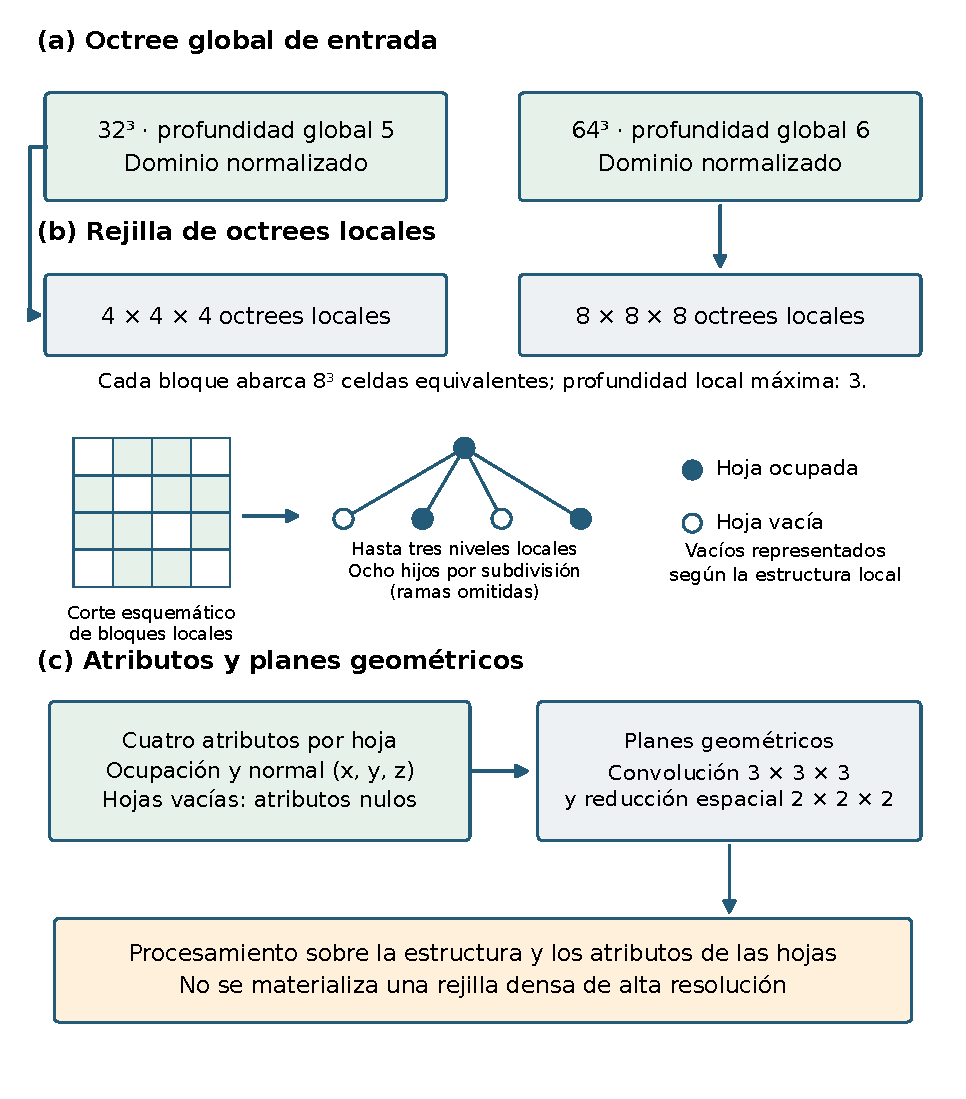
\includegraphics[width=\textwidth,height=0.77\textheight,keepaspectratio]{Figuras/net5_representacion_entrada.pdf}
\caption{Representación de entrada de Net5: (a) resoluciones globales de $32^3$ y $64^3$; (b) rejilla de octrees locales de profundidad máxima tres, con hojas ocupadas y vacías; (c) cuatro atributos por hoja y planes geométricos. No se materializa un tensor denso de alta resolución. Esquema conceptual de elaboración propia conforme a la implementación.}\label{fig:net5-entrada}
\end{figure}

\subsection{Arquitectura y configuración}
\label{subsec:net5-arquitectura}

La red se organizó en cinco bloques, cada uno con dos convoluciones tridimensionales de soporte $3\times3\times3$ y una activación ReLU después de cada convolución. Las operaciones se aplicaron sobre los atributos de las hojas de la representación híbrida. La Tabla~\ref{tab:net5-arquitectura} presenta los canales utilizados y la ubicación de las reducciones espaciales. La distribución de canales y la capa de 512 unidades proceden de la arquitectura de capacidad fija del suplemento de OctNet; los cuatro canales de entrada y las 40 salidas corresponden a la adaptación de este proyecto \parencite{riegler2017}.

\begin{table}[htbp]
\centering\small
\caption{Configuración de los bloques convolucionales de Net5 para ambas resoluciones. Cada flecha indica un cambio en el número de canales. La reducción espacial divide por dos la resolución de cada eje. Elaboración propia a partir de la implementación y de la arquitectura de referencia de OctNet.}
\label{tab:net5-arquitectura}
\begin{tabular}{@{}clcc@{}}
\toprule
Bloque & Canales de las dos convoluciones & Reducción en $32^3$ & Reducción en $64^3$ \\
\midrule
1 & $4\to8\to14$ & No & No \\
2 & $14\to14\to20$ & No & No \\
3 & $20\to20\to26$ & No & Sí \\
4 & $26\to26\to32$ & Sí & Sí \\
5 & $32\to32\to32$ & Sí & Sí \\
\bottomrule
\end{tabular}
\end{table}

La reducción espacial por máximo se aplicó después de los bloques cuarto y quinto en $32^3$, y después de los bloques tercero, cuarto y quinto en $64^3$. En ambos casos, la salida convolucional alcanzó una resolución equivalente de $8^3$ y 32 canales. Esta disposición mantuvo constantes las dimensiones de entrada al clasificador final.

Únicamente al finalizar los cinco bloques se materializó un tensor de $32\times8\times8\times8$ por objeto. Sus $16\,384$ componentes se reorganizaron en un vector; posteriormente se aplicaron una desactivación aleatoria de unidades con probabilidad $0{,}5$, una capa completamente conectada de 512 unidades con ReLU y una capa de salida de 40 unidades. La salida consistió en puntuaciones sin normalización previa; la función de pérdida \texttt{CrossEntropyLoss} recibió directamente estas puntuaciones y las etiquetas. Durante la evaluación se desactivó la desactivación aleatoria de unidades mediante el modo de evaluación del modelo.

La implementación nativa se identificó como \protect\path{octree_native} y utilizó la clase \texttt{Net5Octree} de \protect\path{net5_modelo.py}. Ambas resoluciones tuvieron $8\,547\,456$ parámetros entrenables. La referencia densa disponible en el repositorio constituye una implementación distinta para comprobaciones de equivalencia; no fue la utilizada en las ejecuciones nativas descritas aquí. En consecuencia, la ausencia de expansión densa se refiere al procesamiento convolucional de alta resolución, no al tensor final de $8^3$ utilizado por las capas completamente conectadas.

La Figura~\ref{fig:net5-arquitectura} integra los cinco bloques y muestra dónde difieren las reducciones espaciales entre resoluciones.
\begin{figure}[p]
\centering
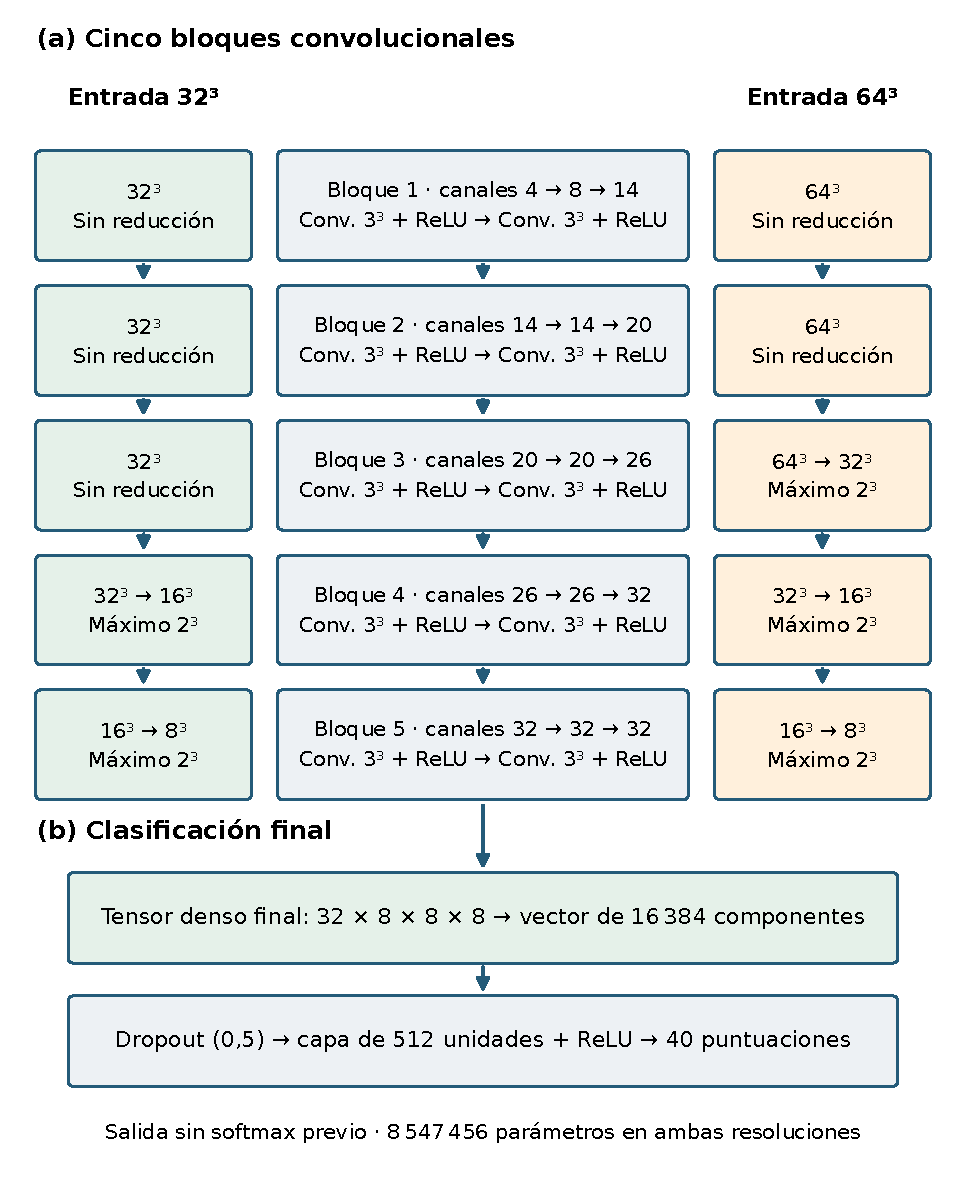
\includegraphics[width=\textwidth,height=0.77\textheight,keepaspectratio]{Figuras/net5_arquitectura.pdf}
\caption{Arquitectura implementada de Net5: (a) cinco bloques y reducciones para $32^3$ y $64^3$; (b) expansión final a baja resolución y clasificador de 40 puntuaciones. Cada bloque contiene dos convoluciones y sus activaciones ReLU. Elaboración propia a partir de la implementación, basada en OctNet \parencite{riegler2017}.}\label{fig:net5-arquitectura}
\end{figure}

\subsection{Entrenamiento, validación y selección del modelo}
\label{subsec:net5-entrenamiento}

Se conservaron los $9\,843$ objetos del entrenamiento oficial y los $2\,468$ objetos de prueba. El entrenamiento oficial se dividió de forma estratificada, con semilla 42, en $8\,858$ objetos para el ajuste de pesos y 985 para validación. El procedimiento de partición se registró en un manifiesto con identificadores de objetos. Para comprobar la correspondencia entre resoluciones, se contrastaron las huellas SHA-256 del manifiesto consignadas en los resúmenes de ambas ejecuciones de Net5.

La correspondencia con HCE se examinó mediante los registros complementarios \protect\path{relacion_filas_hce_R32.csv} y \protect\path{relacion_filas_hce_R64.csv}. Estos relacionan cada fila de la matriz del entrenamiento oficial con un identificador de objeto, su categoría, el subconjunto asignado y la posición dentro de este; además, incluyen la huella SHA-256 del archivo de características. La comprobación contempló el tipo de coincidencia de descriptores registrado para cada fila. Se compararon los identificadores y sus posiciones con las listas completas del manifiesto de Net5, se buscaron identificadores duplicados y se contrastaron las huellas consignadas con las calculadas sobre los NPZ revisados. Se examinó el programa \protect\path{trazabilidad_filas_hce.py},
que vuelve a extraer los descriptores desde los octrees y compara
sus representaciones binarias en \texttt{float32} con las filas
de las matrices HCE almacenadas. El procedimiento distingue
coincidencias únicas, ambiguas y ausentes. Esta verificación es
posterior al entrenamiento y complementa la trazabilidad de los
archivos originales. Durante la revisión documental se examinó
el código y se contrastaron los CSV suministrados con el manifiesto,
sin repetir la extracción sobre los octrees originales. La comparación no modificó las particiones ni los modelos entrenados y no utilizó el conjunto de prueba para seleccionar modelos.

La Tabla~\ref{tab:net5-configuracion} resume la configuración efectiva registrada en los resúmenes de las ejecuciones completas, que se distinguió de los valores predeterminados de la línea de comandos y de las pruebas breves de funcionamiento.

\begin{table}[htbp]
\centering\small
\caption{Configuración común de entrenamiento de Net5 en $32^3$ y $64^3$. Los parámetros adimensionales se indican sin unidades; las cantidades de objetos y épocas son conteos. Elaboración propia a partir de los registros de ejecución.}
\label{tab:net5-configuracion}
\begin{tabularx}{\textwidth}{@{}>{\raggedright\arraybackslash}X>{\raggedright\arraybackslash}X@{}}
\toprule
Parámetro & Valor o procedimiento \\
\midrule
Semilla & 42 \\
Objetos de ajuste / validación / prueba & $8\,858$ / 985 / $2\,468$ \\
Optimizador & Adam \\
Tasa de aprendizaje inicial & $10^{-4}$ \\
Decaimiento de pesos & $10^{-4}$ \\
Plan de tasa de aprendizaje & Factor $0{,}7$ cada 20 épocas \\
Tamaño del lote & 1 objeto \\
Máximo de épocas & 200 \\
Parada anticipada & 20 épocas consecutivas sin mejora estricta de la exactitud de validación \\
Procesos de carga & 8; una muestra anticipada por proceso \\
Preparación geométrica & Precalculada durante la carga \\
\bottomrule
\end{tabularx}
\end{table}

Estos valores se aplicaron por separado a cada resolución. El orden de las muestras de ajuste se barajó mediante un generador inicializado con la semilla indicada; los subconjuntos de validación y prueba se recorrieron sin barajado. Se limitó a uno el número de hilos de las bibliotecas numéricas de CPU indicadas en los registros. Los procesos de carga se conservaron entre recorridos de prueba, pero no entre épocas de ajuste y validación.

La Ecuación~\eqref{eq:net5-perdida} expresa la pérdida de entropía cruzada utilizada para el ajuste a partir de las puntuaciones sin normalizar:
\begin{equation}\label{eq:net5-perdida}
\mathcal L_{\mathrm{CE}}=-\frac{1}{n_{\mathrm{lote}}}\sum_{i=1}^{n_{\mathrm{lote}}}\log\left(\frac{\exp z_{i,y_i}}{\sum_{c=0}^{K-1}\exp z_{i,c}}\right).
\end{equation}
Aquí $n_{\mathrm{lote}}$ es el número de objetos del lote, $K$ el número de categorías, $z_{i,c}$ la puntuación de la red para el objeto $i$ y la categoría $c$, e $y_i$ la etiqueta real, con $c,y_i\in\{0,\ldots,K-1\}$. El símbolo $B$ se reservó para el número de árboles del bosque. La función exponencial transforma las puntuaciones y el denominador normaliza sobre las categorías; el logaritmo es natural. En la configuración utilizada el lote contuvo un objeto y la salida tuvo cuarenta puntuaciones. La implementación recibió directamente las puntuaciones mediante \texttt{CrossEntropyLoss}, que realizó internamente el cálculo numéricamente estable; no se aplicó una normalización adicional antes de la pérdida.

La Ecuación~\eqref{eq:net5-decision} define la etiqueta seleccionada durante la evaluación:
\begin{equation}\label{eq:net5-decision}
\widehat y_i=\operatorname*{arg\,max}_{c\in\{0,\ldots,39\}}z_{i,c}.
\end{equation}
$\widehat y_i$ es la categoría predicha y $z_{i,c}$ conserva el significado anterior. Esta decisión se aplicó sin actualizar parámetros y permitió construir los conteos de validación y prueba. Las puntuaciones se utilizaron para decidir la categoría, sin atribuirles una calibración probabilística comprobada.

En cada época se calcularon las puntuaciones de las muestras de ajuste, la pérdida de entropía cruzada y sus gradientes; a continuación se actualizaron los pesos mediante Adam, que utiliza estimaciones adaptativas de los primeros y segundos momentos de los gradientes~\parencite{kingma2015adam}. Tras recorrer el subconjunto de ajuste, se evaluó el modelo sobre los 985 objetos de validación, sin actualización de pesos. Se registraron la pérdida y la exactitud de ambos subconjuntos y se actualizó la tasa de aprendizaje mediante \texttt{StepLR}.

Se guardó un nuevo estado seleccionado únicamente cuando la exactitud de validación superó estrictamente la mejor exactitud anterior. Un empate no reemplazó el estado conservado y contó como una época sin mejora. El entrenamiento finalizó al alcanzar el máximo de épocas o 20 épocas consecutivas sin mejora. La selección dependió de la exactitud de validación, no de la pérdida de prueba ni de la exactitud de prueba.

Finalizado el ajuste, se recargó el estado seleccionado y se evaluaron los $2\,468$ objetos del conjunto oficial de prueba. Se obtuvieron la exactitud global, la pérdida, la matriz de confusión y el informe por categoría. Para los conteos y métricas por clase se mantuvieron las definiciones de las Ecuaciones~\eqref{eq:hce-verdaderos-positivos}--\eqref{eq:hce-falsos-negativos} y de las Ecuaciones~\eqref{eq:hce-precision-clase}--\eqref{eq:hce-f1-clase}. Los resultados de prueba no se utilizaron para seleccionar la época del modelo.

Se conservaron dos estados por resolución: el de mejor validación y el último estado de entrenamiento. El primero contiene los pesos seleccionados y su configuración; el segundo incorpora además los estados del optimizador, del plan de tasa de aprendizaje y la información necesaria para reanudar una ejecución compatible. El historial por época se escribió en CSV y JSON. Los resúmenes \protect\path{resumen_net5_octree_R32.json} y \protect\path{resumen_net5_octree_R64.json} registraron la configuración, la partición, el entorno, la versión del código y las métricas. Los archivos de pesos y los artefactos de partición se conservaron junto con los registros necesarios para la reevaluación; sus identificadores y comprobaciones se documentaron en el repositorio.

El entorno registrado incluyó Windows 11, Python 3.14.4, PyTorch 2.11.0 con CUDA \texttt{12.8} y una GPU NVIDIA GeForce RTX 5070 de 12 GB. La trazabilidad de las ejecuciones se examinó mediante el identificador de versión \texttt{8164428} y el estado de modificaciones locales consignado en los registros. La integración posterior del código y de los registros se revisó en la versión \texttt{64b8835}; esta revisión documental no constituyó una repetición del entrenamiento.

En los registros, el tiempo acumulado de entrenamiento corresponde a la suma de los intervalos de las épocas, que incluyeron ajuste, validación y actualización del plan de tasa de aprendizaje. Quedaron fuera de dichos intervalos la escritura posterior de los estados y la evaluación final. Por ello, esta magnitud no se interpretó como la duración completa del programa. Asimismo, la llamada de inferencia del modelo nativo puede incluir preparación y transferencia de planes internos. Su alcance se debe distinguir del tiempo de predicción de HCE sobre características previamente calculadas al desarrollar la comparación experimental.


La Figura~\ref{fig:net5-entrenamiento} distingue la actualización de pesos, la selección mediante validación y la evaluación final del estado conservado.
\begin{figure}[p]
\centering
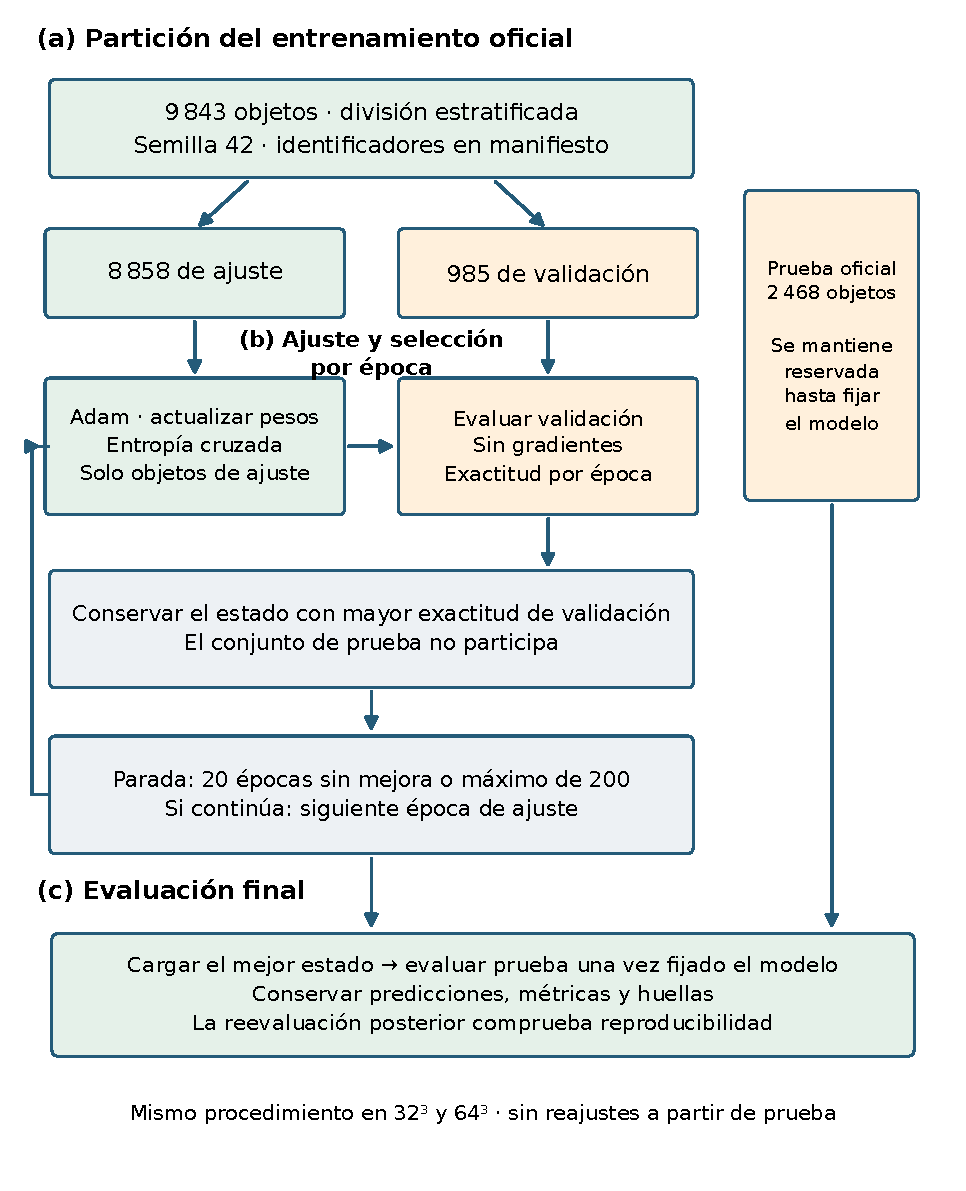
\includegraphics[width=\textwidth,height=0.77\textheight,keepaspectratio]{Figuras/net5_entrenamiento.pdf}
\caption{Entrenamiento y selección de Net5 en ambas resoluciones: (a) partición del entrenamiento oficial; (b) ajuste con Adam, validación por época y selección del mejor estado; (c) evaluación final sobre los $2\,468$ objetos oficiales de prueba. La prueba no interviene en la elección del modelo. Elaboración propia.}\label{fig:net5-entrenamiento}
\end{figure}

\FloatBarrier
\section{Protocolo experimental y trazabilidad}
\label{sec:protocolo-experimental}

Esta sección establece el protocolo empleado para comparar las representaciones y los clasificadores desarrollados en las etapas anteriores. Se describen el diseño experimental, el alcance de los conjuntos de datos, los criterios de equivalencia, las métricas de desempeño y costo, el análisis estadístico y las medidas adoptadas para garantizar la reproducibilidad y trazabilidad de los resultados. El protocolo se aplicó a los modelos previamente seleccionados, sin efectuar nuevos ajustes a partir del conjunto oficial de prueba. La Figura~\ref{fig:protocolo-comparacion} sintetiza las entradas, las ramas de evaluación y las verificaciones que sustentan la comparación por método y resolución.

\begin{figure}[p]
\centering
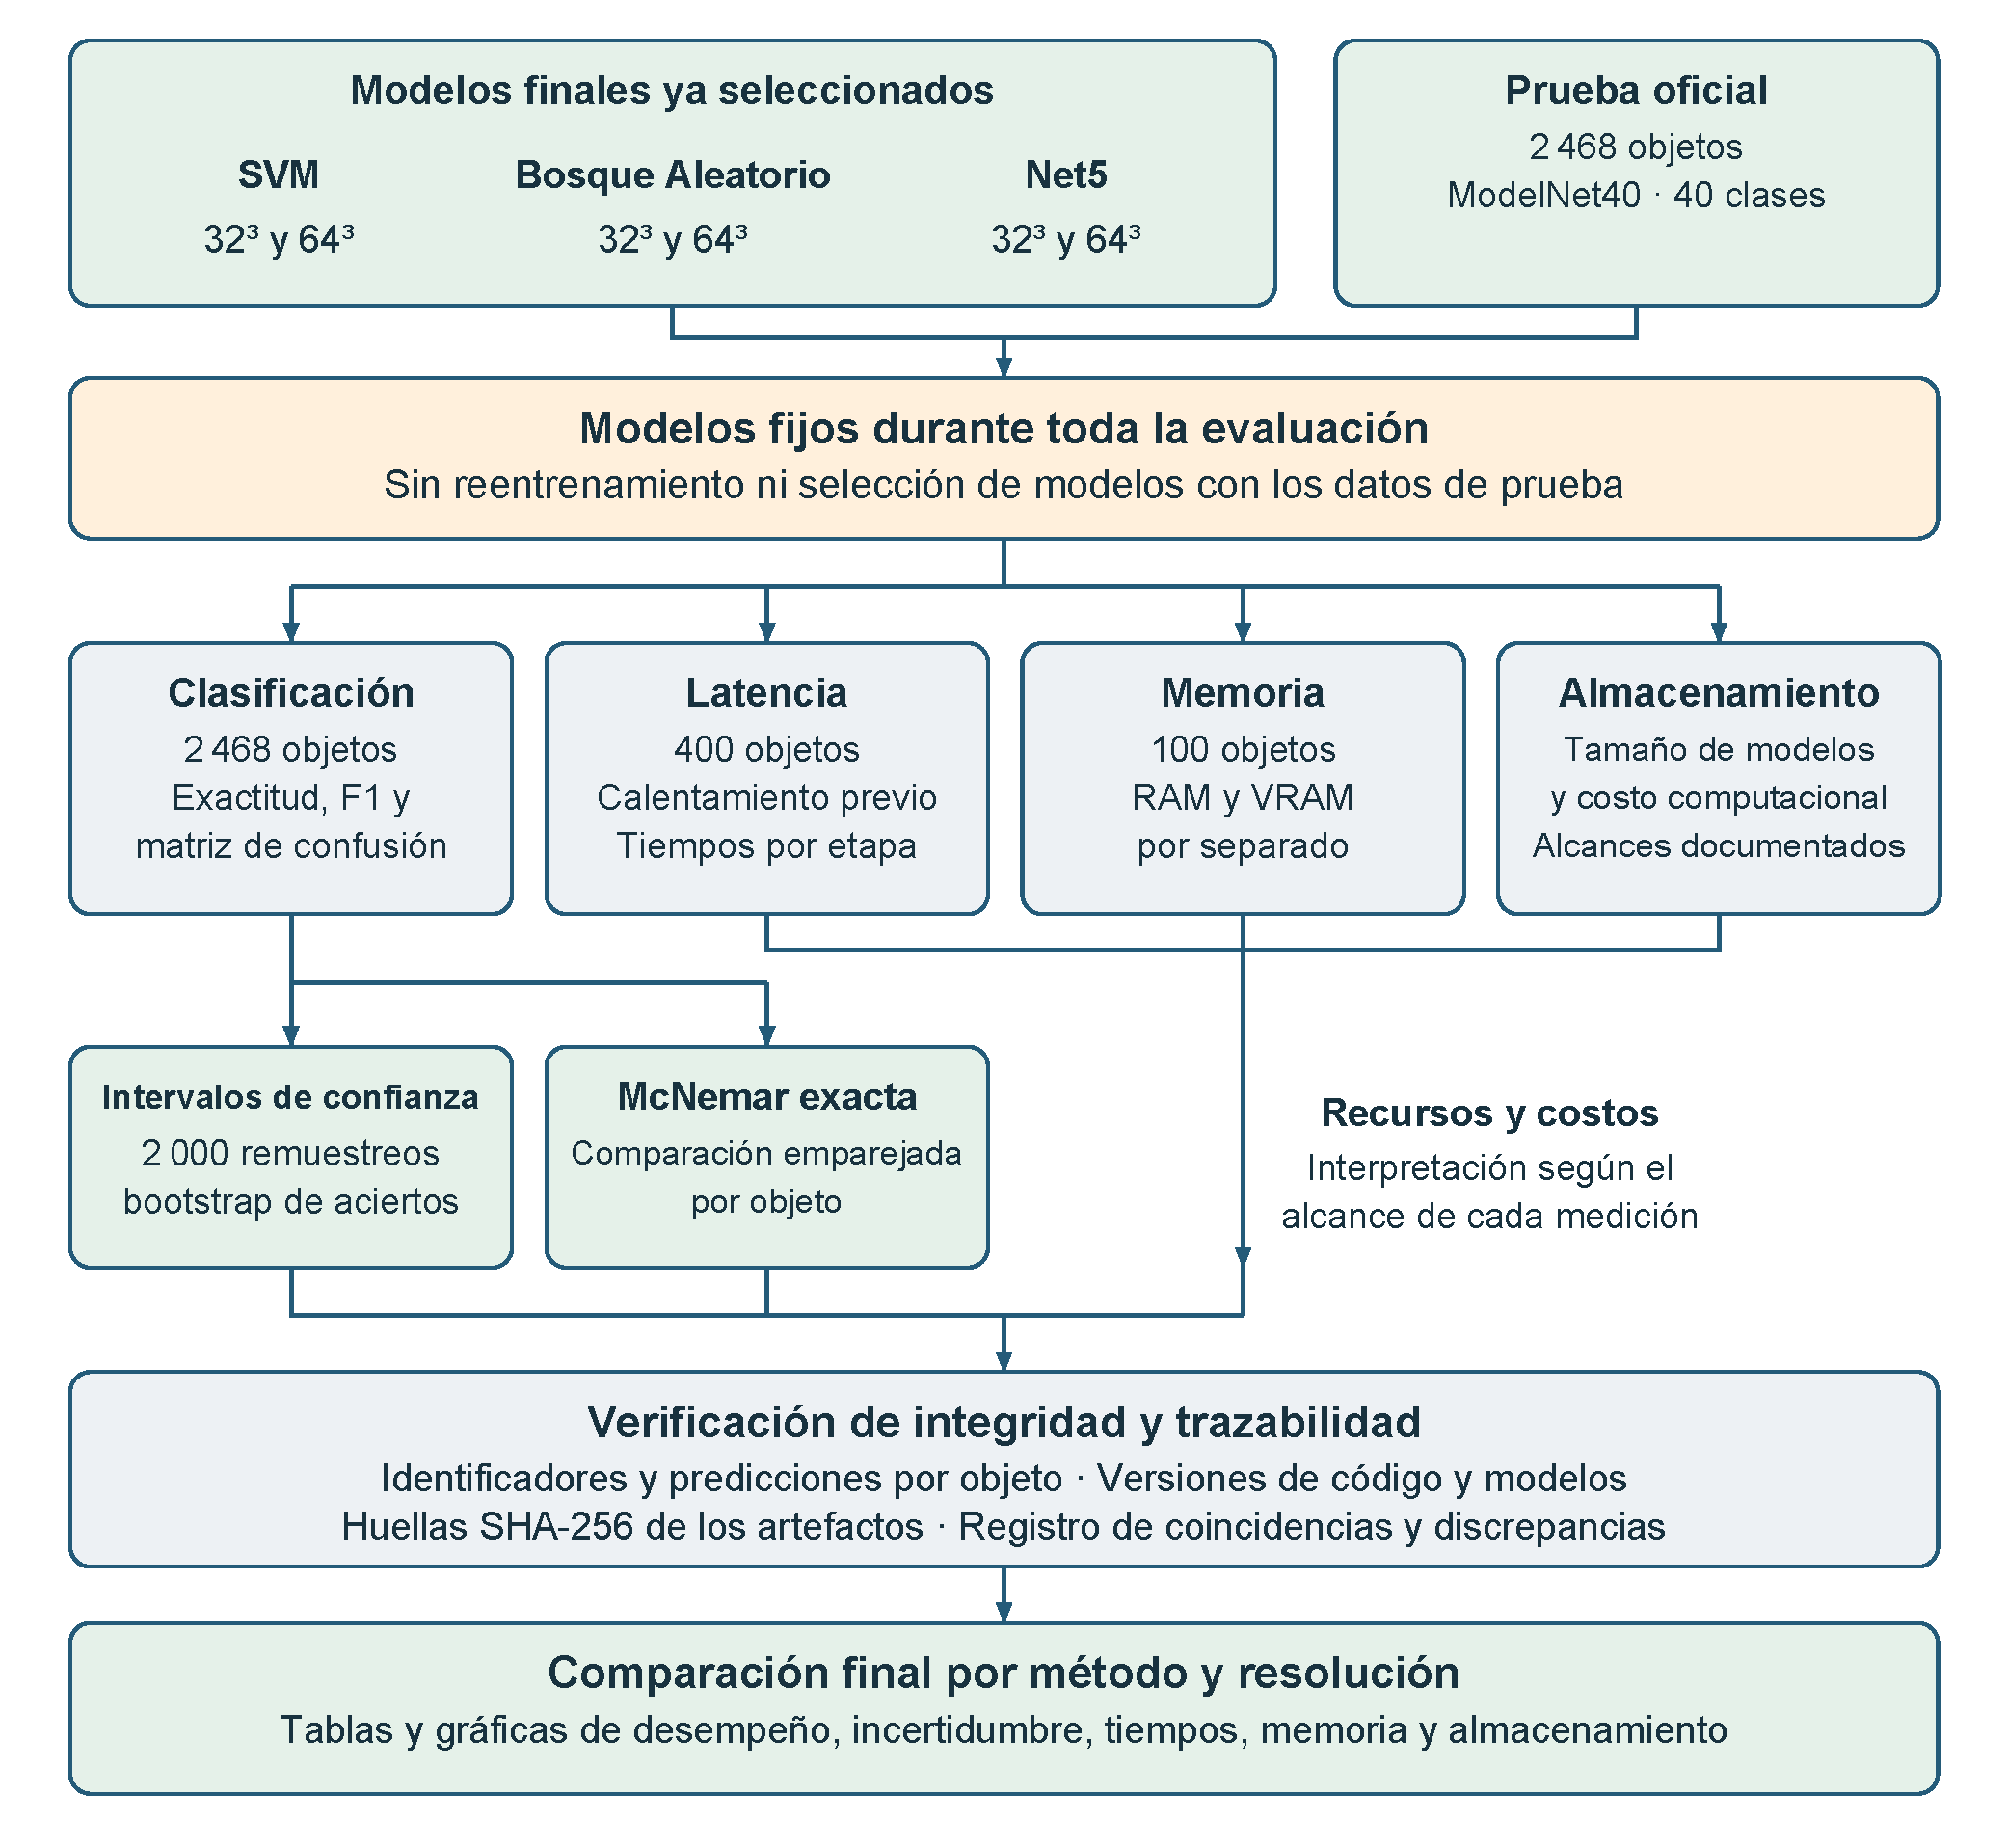
\includegraphics[width=\textwidth]{Figuras/protocolo_comparacion.pdf}
\caption{Flujo de evaluación de los modelos finales SVM, Bosque Aleatorio y Net5 en resoluciones equivalentes de $32^3$ y $64^3$. El conjunto oficial de prueba contiene $2\,468$ objetos y no interviene en el reentrenamiento ni en la selección de modelos. La clasificación alimenta los intervalos de confianza mediante $2\,000$ remuestreos \textit{bootstrap} y las comparaciones emparejadas mediante la prueba exacta de McNemar; la latencia se mide sobre 400 objetos y la memoria sobre 100. Los recursos se interpretan según el alcance de cada medición y los artefactos se someten a comprobaciones de integridad y trazabilidad antes de consolidar la comparación. Elaboración propia.}
\label{fig:protocolo-comparacion}
\end{figure}

\subsection{Diseño general de la investigación}
\label{subsec:diseno-investigacion}
Se realizó un estudio experimental comparativo con tres clasificadores y dos resoluciones. Se mantuvieron fijos el conjunto de datos, la semilla de referencia y la definición de las etiquetas. Se distinguieron tres actividades: la comprobación geométrica del primer objetivo, el entrenamiento y selección de los modelos de los objetivos segundo y tercero, y la evaluación comparativa de los modelos conservados. La construcción y validación geométrica correspondieron al primer objetivo; HCE y los clasificadores tradicionales, al segundo; y Net5, al tercero. El protocolo reproducible, las configuraciones y la trazabilidad correspondieron al cuarto objetivo; la comparación de clasificación, el análisis de costos y el compromiso por resolución, al quinto. No se reentrenaron modelos durante la comparación final.

La evaluación principal se obtuvo de los archivos versionados en \protect\path{resultados/Objetivos_4_y_5_comparacion}. Se examinó separadamente la reevaluación del 27 de septiembre de 2026, registrada en \protect\path{resultados/Objetivos_4_y_5_reevaluacion_2026-09-27}. El protocolo de esta segunda evaluación contempló la comparación, por identificador, de las predicciones conservadas y las recalculadas, así como el registro de tiempos y memoria bajo las condiciones documentadas de cada ejecución. No constituyó una repetición del entrenamiento con otra semilla.

\subsection{Conjunto de datos y preparación experimental}
\label{subsec:datos-preparacion}
Se respetó la separación oficial entre los $9\,843$ objetos de entrenamiento y los $2\,468$ de prueba. Los modelos seleccionados se evaluaron sobre todos los objetos de prueba, con 40 categorías. Para Net5 se cargaron los octrees desde los archivos NPZ. Para los clasificadores clásicos se utilizaron las características conservadas; en la medición de latencia se regeneraron los descriptores desde los octrees de la muestra y se contrastaron sus predicciones. Por tanto, la reevaluación de HCE no se presentó como una regeneración completa de todas las características desde las mallas originales.

Se definieron muestras diferentes según la magnitud observada. La comprobación geométrica utilizó los diez objetos y veinte registros modelo--resolución descritos en la Sección~\ref{sec:construccion-representaciones}. La clasificación utilizó los $2\,468$ objetos. La latencia utilizó 400 objetos por resolución, diez por categoría, después de diez objetos de calentamiento excluidos del resumen. La memoria se midió sobre cien objetos. La selección efectiva de estos últimos incluyó cuarenta objetos de \texttt{airplane}, cuarenta de \texttt{bathtub} y veinte de \texttt{bed}; no fue una muestra equilibrada de las cuarenta clases.

\subsection{Criterios de equivalencia experimental}
\label{subsec:equivalencia-experimental}
Las comparaciones de clasificación se emparejaron por identificador de objeto, etiqueta y resolución. Se conservaron los modelos seleccionados mediante validación; las etiquetas de prueba no intervinieron en la selección de hiperparámetros ni de épocas. La implementación de SVM incluyó el escalado dentro del procedimiento de entrenamiento, ajustado exclusivamente con los datos del pliegue correspondiente.

La medición de latencia se realizó objeto a objeto, con un solo proceso, sin procesos de carga y con un hilo de las bibliotecas de CPU. El bosque aleatorio se evaluó con \protect\path{n_jobs=1}. Estas condiciones difieren de los ocho procesos de carga empleados en el entrenamiento de Net5. Se registraron intervalos mediante \protect\path{perf_counter}; cada objeto aportó una observación por caso y ejecución. Se informaron la media, la mediana y el percentil 95 de esas observaciones, sin confundir 400 objetos con 400 repeticiones del mismo objeto.

Para HCE, el tiempo agregado incluyó la carga del NPZ, la extracción y adecuación de características y la predicción. En SVM, la predicción incluyó la transformación mediante el escalador conservado. Para Net5 se midieron la carga, la conversión geométrica y preparación de planes, y la propagación de la red. La implementación de la medición GPU dejó fuera el armado del lote anterior a la propagación; en CPU, ese armado quedó incluido en el intervalo de propagación. Esta asimetría se conservó explícita al interpretar los resultados. Los tiempos comenzaron en el NPZ y no incluyeron la lectura OFF ni la construcción inicial del octree. Tampoco se sumaron medianas de componentes para obtener la mediana total: primero se sumaron los intervalos de cada objeto y después se resumieron los totales.

Para memoria se creó un proceso independiente por caso. Se tomó una base después de importar las bibliotecas y se muestreó el conjunto de trabajo de Windows cada 2 ms durante la inferencia. Las Ecuaciones~\eqref{eq:memoria-pico}--\eqref{eq:memoria-incremento} definen el pico observado y su incremento sobre la base:
\begin{subequations}\label{eq:memoria-comparacion}
\begin{align}
M_{\mathrm{pico}}&=\max_{t\in\mathcal{T}}M(t),\label{eq:memoria-pico}\\
\Delta M&=M_{\mathrm{pico}}-M_{\mathrm{base}}.\label{eq:memoria-incremento}
\end{align}
\end{subequations}
Aquí $M(t)$ es la memoria residente observada en el instante $t$, $\mathcal{T}$ es el conjunto de instantes muestreados y $M_{\mathrm{base}}$ es la memoria inicial del proceso. Todas estas magnitudes se expresaron en MiB, con $2^{20}$ bytes por unidad. El incremento incluyó la carga del modelo y los recursos posteriores; no representó exclusivamente sus parámetros. El muestreo temporal puede omitir picos más breves que su intervalo. La memoria asignada y reservada por PyTorch en GPU se informó por separado y no se sumó a la RAM como si fueran una única magnitud.

Se distinguió el tamaño de los modelos en disco, expresado en MB decimales, de la memoria residente y de las estimaciones binarias de la representación. El tiempo de extracción HCE para entrenamiento se estimó extrapolando la media de carga y extracción de la muestra a $9\,843$ objetos. Se identificó como estimación y no como un cronometraje de la ejecución completa. Los tiempos de ajuste de SVM incluyeron la búsqueda de hiperparámetros, los del bosque correspondieron a su ajuste y los de Net5 a los intervalos acumulados por época; estas magnitudes no tienen idéntico alcance.

\subsection{Métricas y análisis estadístico}
\label{subsec:metricas-analisis}
Se construyó la matriz de confusión definida en la Ecuación~\eqref{eq:hce-matriz-confusion}, con las categorías reales en las filas y las predichas en las columnas. Para las figuras se utilizó la normalización por fila definida en la Ecuación~\eqref{eq:confusion-final}:
\begin{equation}\label{eq:confusion-final}
\widetilde M_{c,j}=\frac{M_{c,j}}{\sum_{k=0}^{39}M_{c,k}}.
\end{equation}
$M_{c,j}$ es el número de objetos de categoría real $c$ predichos como $j$, $k$ recorre las columnas y $\widetilde M_{c,j}$ es la proporción correspondiente dentro de la categoría real. Todas las categorías tuvieron soporte positivo. Esta transformación permitió comparar categorías con soportes diferentes; los conteos originales se conservaron para los contrastes emparejados.

Las Ecuaciones~\eqref{eq:exactitud-global-final}--\eqref{eq:f1-ponderado-final} definen la exactitud global, la exactitud balanceada y los dos promedios de $F_1$ utilizados:
\begin{subequations}\label{eq:metricas-agregadas}
\begin{align}
A&=\frac{1}{n_{\mathrm{test}}}\sum_{c=0}^{39}M_{c,c}, \label{eq:exactitud-global-final} \\
A_{\mathrm{bal}}&=\frac{1}{40}\sum_{c=0}^{39}S_c, \label{eq:exactitud-balanceada-final} \\
F_{1,\mathrm{macro}}&=\frac{1}{40}\sum_{c=0}^{39}F_{1,c}, \label{eq:f1-macro-final} \\
F_{1,\mathrm{pond}}&=\frac{1}{n_{\mathrm{test}}}\sum_{c=0}^{39}n_c F_{1,c}. \label{eq:f1-ponderado-final}
\end{align}
\end{subequations}
Aquí $n_{\mathrm{test}}$ es el número de objetos de prueba; $S_c$ es la sensibilidad de la categoría $c$, $F_{1,c}$ su F1 y $n_c$ su soporte. Las definiciones por clase se presentaron en las Ecuaciones~\eqref{eq:hce-verdaderos-positivos}--\eqref{eq:hce-falsos-negativos} y en las Ecuaciones~\eqref{eq:hce-precision-clase}--\eqref{eq:hce-f1-clase}. Las métricas son adimensionales y se expresaron como porcentajes en las tablas. El promedio macro asigna el mismo peso a cada categoría; el ponderado asigna pesos proporcionales a sus soportes. Esta distinción permitió examinar el efecto de las clases con menos objetos de prueba.

Para estimar intervalos de la exactitud de un modelo fijo se utilizó el método de remuestreo con reemplazo o \textit{bootstrap}, empleado para aproximar la variabilidad estadística y construir intervalos de confianza~\parencite{efron1986bootstrap}. Se calcularon intervalos percentiles mediante 2\,000 remuestreos con reemplazo de los indicadores de acierto de prueba, con semilla 42. La Ecuación~\eqref{eq:ic-remuestreo} expresa el intervalo empleado:
\begin{equation}\label{eq:ic-remuestreo}
I_{95}=\left[Q_{0{,}025}\!\left(\{A^{*(b)}\}_{b=1}^{J}\right),\ Q_{0{,}975}\!\left(\{A^{*(b)}\}_{b=1}^{J}\right)\right].
\end{equation}
$A^{*(b)}$ es la exactitud del remuestreo $b$, $J$ es el número de remuestreos y $Q_q$ el cuantil de orden $q$. Cada remuestreo conservó el número de objetos del conjunto de prueba. Estos intervalos describen la variación asociada al remuestreo de ese conjunto para un modelo fijo; no cuantifican la variabilidad entre entrenamientos ni entre semillas.

La comparación de aciertos emparejados se fundamentó en la prueba de McNemar para proporciones correlacionadas~\parencite{mcnemar1947}. Se empleó su variante exacta condicional, que calcula la probabilidad de los pares discordantes mediante una distribución binomial bajo la hipótesis nula~\parencite{fagerland2013}. La implementación utilizó la función \texttt{binomtest} de SciPy con alternativa bilateral~\parencite{scipybinom}. Las Ecuaciones~\eqref{eq:mcnemar-discordantes}--\eqref{eq:mcnemar-probabilidad} muestran el cálculo para los pares discordantes:
\begin{subequations}\label{eq:mcnemar-final}
\begin{align}
d&=u+v, \label{eq:mcnemar-discordantes} \\
h&=\min(u,v), \label{eq:mcnemar-minimo} \\
p&=\min\left(1,\ 2\sum_{j=0}^{h}\binom{d}{j}2^{-d}\right). \label{eq:mcnemar-probabilidad}
\end{align}
\end{subequations}
$u$ cuenta los objetos acertados únicamente por el primer método, $v$ los acertados únicamente por el segundo, $d$ el total de discordancias y $p$ el valor de probabilidad bilateral bajo igualdad de las probabilidades discordantes. Si no existieron discordancias se asignó un valor de probabilidad unitario. Se realizaron nueve contrastes: tres pares de métodos por resolución y tres pares de resoluciones por método. El umbral nominal fue $0{,}05$ y no se aplicó ajuste por comparaciones múltiples. Por ello, los resultados se interpretaron como contrastes individuales exploratorios; la ausencia de significación no se interpretó como equivalencia entre modelos.

Para estudiar la resolución, las Ecuaciones~\eqref{eq:cambio-exactitud}--\eqref{eq:razon-costos} definen la diferencia de exactitud y la razón de costos:
\begin{subequations}\label{eq:cambio-resolucion}
\begin{align}
\Delta A&=100\left(A_{64}-A_{32}\right), \label{eq:cambio-exactitud} \\
\rho_X&=\frac{X_{64}}{X_{32}}. \label{eq:razon-costos}
\end{align}
\end{subequations}
$\Delta A$ se expresa en puntos porcentuales; $A_{32}$ y $A_{64}$ son exactitudes expresadas como fracciones. $X$ representa una magnitud positiva de costo medida con el mismo protocolo en ambas resoluciones y $\rho_X$ es adimensional. Se utilizaron estas cantidades para valorar los aciertos adicionales frente al aumento de latencia, almacenamiento y entrenamiento.

\subsection{Entorno computacional, reproducibilidad y trazabilidad}
\label{subsec:entorno-reproducibilidad}
La comparación se ejecutó en Windows 11, con 16 procesadores lógicos, aproximadamente 32 GB de RAM y una NVIDIA GeForce RTX 5070 de 12 GB. Los registros identificaron el procesador como \texttt{AMD64 Family 25 Model 33 Stepping 0}; esta identificación automática se conservó sin inferir un modelo comercial más específico. Se registraron Python 3.14.4, NumPy 2.4.6, scikit-learn 1.9.0 y PyTorch 2.11.0 con CUDA 12.8. Las versiones se informan como parte del entorno registrado en los experimentos.

Se conservaron las predicciones por objeto, los tiempos individuales, los resúmenes, las configuraciones, los modelos seleccionados y las huellas de los artefactos. Los programas \protect\path{fase4_comparacion/evaluar_comparacion.py}, \protect\path{fase4_comparacion/auditar_comparacion.py}, \protect\path{fase4_comparacion/tablas_comparacion.py} y \protect\path{fase4_comparacion/figuras_comparacion.py} organizaron la evaluación, las comprobaciones y los productos de presentación. Las instrucciones de preparación y ejecución se documentaron en los archivos de descripción del repositorio.

El entrenamiento de Net5 quedó asociado a la versión \texttt{8164428}; la reevaluación del 27 de septiembre registró \texttt{8147a6e}. La revisión documental utilizó el estado consolidado \texttt{64b8835} del repositorio. Se distinguieron estas versiones porque integrar resultados posteriormente no cambia la versión con la que fueron obtenidos. Para cada combinación de método y resolución se contrastaron las secuencias de predicciones y se revisó el informe de pruebas automatizadas de la ejecución. Los resultados de estas comprobaciones se presentan en el capítulo de resultados. La revisión documental se distinguió de una nueva ejecución local de los experimentos.
